%\documentclass[a4paper,12pt,twoside]{book}
\documentclass[12pt,times]{report}
\usepackage{mathptmx}%This package supersedes times and mathptm
\usepackage[a4paper,right=2.54cm,left=2.54cm,top=2.54cm,bottom=2.54cm]{geometry}

%%%%paquete para usar citas de diferentes formatos
%%%%%%%%%%%%%%%%%%%%%%%%%%%%%%%%%
%%add al indice
%\usepackage[nottoc,numbib]{tocbibind}
%\usepackage[authoryear,round]{natbib}
\usepackage[utf8]{inputenc}
\usepackage{csquotes}
\usepackage[spanish]{babel}
\usepackage[style=apa ,
%hyperref=auto,
%citestyle=authoryear,
natbib=true,
backend=biber]{biblatex}
\addbibresource{biblio/references.bib}
\usepackage{biblatex}
%paquete para hiperlinks entre citas e imagenes
%%%%%%%%%%%%%%%%%%%%%%%%%%%%%%%%%
\usepackage[colorlinks=true,
citecolor=blue,
urlcolor=cyan,
bookmarks=true,
linkcolor=blue,
pdftitle={Tesis-nombre-alumno},
pdfauthor={autor nombres}]{hyperref}

\usepackage{amssymb}
\usepackage{graphicx} % for improved inclusion of graphics
%\usepackage{wrapfig} % to include figure with text wrapping around it
\usepackage[margin=10pt,font=small,labelfont=bf]{caption} % for improved layout of figure captions with extra margin, smaller font than text
\usepackage{eucal}
\usepackage[usenames, dvipsnames]{color}
\usepackage[perpage]{footmisc}
%\usepackage[round, sort]{natbib}
\usepackage{ifthen}
\usepackage{multicol} % for pages with multiple text columns, e.g. References
\setlength{\columnsep}{20pt} % space between columns; default 10pt quite narrow
\usepackage[nottoc]{tocbibind} % correct page numbers for bib in TOC, nottoc suppresses an entry for TOC itself
\usepackage{appendix}

%%%----Modificar encabezado y pie de pagina
%%%%%%%%%%%%%%%%%%%%%%%%%%%%%%%%%%%%%%%%%%%%%%%%%%%%%%%%%%%%%%%%%%%%%
\usepackage{fancyhdr} % for better header layout
\newcommand{\changefont}{%
	\fontsize{9pt}{1.5pt}\selectfont
}
\pagestyle{fancy}
\fancyhf{} %% delete default configuration of page
%%\setlength\headheight{15pt}
\fancyhead[L]{\changefont Desarrollo de un Algoritmo de aprendizaje profundo para detectar rutas seguras de las calles de los Ángeles}
\fancyhead[R]{\changefont \leftmark}
%%\fancyfoot[L]{\leftmark}
\fancyfoot[R]{\thepage}

%%%%%%%%%%%%%%%%%%%%%%%%%%%%%5
%%%% Configuracion de los parrafos
%\usepackage{setspace}
%\onehalfspacing
%\linespread{1.25} 
\setlength{\parindent}{0.5in} %%sangria
\setlength{\parskip}{3mm}  %%espacio entre parrafos
\linespread{1.3} %This equals 1.5 linespacing in Word
%%%% nuevo parrafo
%%%%%%%%%%%%%%%%%%%%%%%%%%%%%5
%%%% Centrar valores de una tabla
\usepackage{array}
%%CENTRADO HORIZONTAL
\newcolumntype{P}[1]{>{\centering\arraybackslash}p{#1}}
%%CENTRADO VERTICAL
\newcolumntype{M}[1]{>{\centering\arraybackslash}m{#1}}

%%%%%%%%%%%%%%%%%%%%%%%%%%%%%5
%%%%Paquete para alinear texto
\usepackage{ragged2e}
\usepackage{multirow}
\usepackage{makecell}
\usepackage{rotating}
\usepackage{siunitx} % To align the numbers later on
\usepackage[table,xcdraw]{xcolor}
\usepackage{color, colortbl}
\definecolor{Gray}{gray}{0.9}
\definecolor{orange}{rgb}{1,0.647,0}
\definecolor{turq3}{rgb}{0.54, 0.81, 0.94}
\definecolor{turq}{rgb}{0.63, 0.79, 0.95}
\definecolor{bluejean}{rgb}{0.03, 0.27, 0.49}

%%%%%%%%%%%%%%%%%%%%%%%%%
\usepackage{xparse}
\usepackage{expl3}
%%%%funcion de reemplazar regex
\ExplSyntaxOn
\NewDocumentCommand{\replace}{mmm}
{
	\marian_replace:nnn {#1} {#2} {#3}
}

\tl_new:N \l_marian_input_text_tl
\tl_new:N \l_marian_search_tl
\tl_new:N \l_marian_replace_tl

\cs_new_protected:Npn \marian_replace:nnn #1 #2 #3
{
	\tl_set:Nn \l_marian_input_text_tl { #1 }
	\tl_set:Nn \l_marian_search_tl { #2 }
	\tl_set:Nn \l_marian_replace_tl { #3 }
	\regex_replace_all:nnN { \b\u{l_marian_search_tl}\b } { \u{l_marian_replace_tl} } \l_marian_input_text_tl
	\tl_use:N \l_marian_input_text_tl
}
\ExplSyntaxOff

%%%%%%%%%%%%%%%%%%%%%%%%%%%%%%%%%%%%%%
\usepackage{amsmath}
\numberwithin{equation}{chapter} %%enumerar ecuaciones
\renewcommand{\theequation}{Ecuación \thechapter.\arabic{equation}}   
\usepackage{mathtools, nccmath, cool}
%%%Configuraciones de biblatex

%%hel
%%%%\citeauthor
\makeatletter

%%%%%%%%%%%%
\DeclareCiteCommand{\citeauthor}
{\boolfalse{citetracker}%
	\boolfalse{pagetracker}%
	\usebibmacro{prenote}}
{\ifciteindex
	{\indexnames{labelname}}
	{}%
	\printtext[bibhyperref]{\printnames{labelname}}}
{\multicitedelim}
{\usebibmacro{postnote}}


\DeclareCiteCommand{\citetitle}
{\boolfalse{citetracker}%
	\boolfalse{pagetracker}%
	\usebibmacro{prenote}}
{\ifciteindex
	{\indexfield{indextitle}}
	{}%
	\printtext[bibhyperref]{\printfield[citetitle]{labeltitle}}}
{\multicitedelim}
{\usebibmacro{postnote}}

\DeclareCiteCommand{\cite}
{\usebibmacro{prenote}}
{\usebibmacro{citeindex}%
	\printtext[bibhyperref]{\usebibmacro{cite}}}
{\multicitedelim}
{\usebibmacro{postnote}}

\DeclareCiteCommand*{\cite}
{\usebibmacro{prenote}}
{\usebibmacro{citeindex}%
	\printtext[bibhyperref]{\usebibmacro{citeyear}}}
{\multicitedelim}
{\usebibmacro{postnote}}

\DeclareCiteCommand{\parencite}[\mkbibparens]
{\usebibmacro{prenote}}
{\usebibmacro{citeindex}%
	\printtext[bibhyperref]{\usebibmacro{cite}}}
{\multicitedelim}
{\usebibmacro{postnote}}

\DeclareCiteCommand*{\parencite}[\mkbibparens]
{\usebibmacro{prenote}}
{\usebibmacro{citeindex}%
	\printtext[bibhyperref]{\usebibmacro{citeyear}}}
{\multicitedelim}
{\usebibmacro{postnote}}

\DeclareCiteCommand{\footcite}[\mkbibfootnote]
{\usebibmacro{prenote}}
{\usebibmacro{citeindex}%
	\printtext[bibhyperref]{ \usebibmacro{cite}}}
{\multicitedelim}
{\usebibmacro{postnote}}

\DeclareCiteCommand{\footcitetext}[\mkbibfootnotetext]
{\usebibmacro{prenote}}
{\usebibmacro{citeindex}%
	\printtext[bibhyperref]{\usebibmacro{cite}}}
{\multicitedelim}
{\usebibmacro{postnote}}

\DeclareCiteCommand{\textcite}
{\boolfalse{cbx:parens}}
{\usebibmacro{citeindex}%
	\printtext[bibhyperref]{\usebibmacro{textcite}}}
{\ifbool{cbx:parens}
	{\bibcloseparen\global\boolfalse{cbx:parens}}
	{}%
	\multicitedelim}
{\usebibmacro{textcite:postnote}}
\makeatother
\makeatletter
\let\abx@macro@citeOrig\abx@macro@cite
\renewbibmacro{cite}{%
	\bibhyperref{%
		\let\bibhyperref\relax\relax%
		\abx@macro@citeOrig%
	}%
}
\let\abx@macro@textciteOrig\abx@macro@textcite
\renewbibmacro{textcite}{%
	\bibhyperref{%
		\let\bibhyperref\relax\relax%
		\abx@macro@textciteOrig%
	}%
}%

\makeatother

%%%%%%%%%%%%%%%%%%%%%%%%%%%%%%%%%%%%%%%%%%%
\begin{document}

\begin{titlepage}

	\begin{center}
		%%%cargar imagen
	    
\includegraphics[width=0.45\textwidth]{images_repo/esanlogomin}
		\vspace*{2cm} \\
		UNIVERSIDAD ESAN \vspace*{1ex} \\
		FACULTAD DE INGENIERÍA \vspace*{1ex} \\
		INGENIERÍA DE TECNOLOGÍAS DE INFORMACIÓN Y SISTEMAS\vspace*{8ex} \\
		\textbf{Desarrollo de un Algoritmo de aprendizaje profundo para detectar rutas seguras de las calles de los Ángeles}
		\vspace*{8ex}\\	
		Trabajo de investigación para el curso de Trabajo de Tesis I 
		\vspace*{8ex} \\	
		Nombre Guillermo Díaz Beltrán \\
		Asesor: Marks Calderón		
		\vfill
		
		Lima, \today 
		
	\end{center}
\end{titlepage}
%%cambiar nombres de objetos para el indice y otros
\renewcommand{\listfigurename}{Índice de Figuras}
\renewcommand{\tablename}{Tabla}
\renewcommand{\listtablename}{Índice de Tablas}

%\thispagestyle{plain}
\begin{center}
	\vspace*{1.5cm}
	{\Large \bfseries  Resumen}
\end{center}
\vspace{0.5cm}
Lorem ipsum dolor sit amet, consectetur adipiscing elit, sed do eiusmod tempor incididunt ut labore et dolore magna aliqua. Ac odio tempor orci dapibus ultrices in iaculis nunc sed. Vivamus arcu felis bibendum ut tristique et egestas quis ipsum. Odio morbi quis commodo odio aenean sed adipiscing diam donec. Donec ultrices tincidunt arcu non sodales neque sodales ut. Fusce ut placerat orci nulla pellentesque dignissim enim sit amet. Facilisi etiam dignissim diam quis enim lobortis. Sit amet justo donec enim diam vulputate ut pharetra. Gravida in fermentum et sollicitudin ac orci phasellus egestas. Ultricies tristique nulla aliquet enim tortor at auctor. Nullam vehicula ipsum a arcu cursus vitae congue mauris. Convallis posuere morbi leo urna molestie at elementum eu facilisis. Elit at imperdiet dui accumsan sit amet nulla. Amet consectetur adipiscing elit pellentesque habitant morbi tristique senectus et. Mauris in aliquam sem fringilla ut morbi. Ultricies integer quis auctor elit sed vulputate mi sit. Nulla pellentesque dignissim enim sit amet venenatis urna cursus eget. Ac feugiat sed lectus vestibulum mattis ullamcorper. Eu augue ut lectus arcu bibendum. Rhoncus dolor purus non enim praesent elementum. 

Nulla facilisi cras fermentum odio eu feugiat pretium. Massa massa ultricies mi quis hendrerit. Id leo in vitae turpis massa sed elementum. Quis vel eros donec ac odio tempor orci. Netus et malesuada fames ac turpis egestas integer eget aliquet. Velit ut tortor pretium viverra suspendisse potenti. Ut enim blandit volutpat maecenas. Nibh tellus molestie nunc non blandit. Mus mauris vitae ultricies leo integer malesuada nunc vel. Vel elit scelerisque mauris pellentesque pulvinar pellentesque habitant. Neque viverra justo nec ultrices dui sapien eget. Vitae aliquet nec ullamcorper sit. Dui id ornare arcu odio ut sem nulla pharetra diam. Et magnis dis parturient montes. Varius morbi enim nunc faucibus.
\newline

\textbf{Palabras claves: } uno, dos, tres, cuatro
%\thispagestyle{plain}
\begin{center}
	\vspace*{1.5cm}
	{\Large \bfseries  Abstract}
\end{center}
\vspace{0.5cm}
Lorem ipsum dolor sit amet, consectetur adipiscing elit, sed do eiusmod tempor incididunt ut labore et dolore magna aliqua. Ac odio tempor orci dapibus ultrices in iaculis nunc sed. Vivamus arcu felis bibendum ut tristique et egestas quis ipsum. Odio morbi quis commodo odio aenean sed adipiscing diam donec. Donec ultrices tincidunt arcu non sodales neque sodales ut. Fusce ut placerat orci nulla pellentesque dignissim enim sit amet. Facilisi etiam dignissim diam quis enim lobortis. Sit amet justo donec enim diam vulputate ut pharetra. Gravida in fermentum et sollicitudin ac orci phasellus egestas. Ultricies tristique nulla aliquet enim tortor at auctor. Nullam vehicula ipsum a arcu cursus vitae congue mauris. Convallis posuere morbi leo urna molestie at elementum eu facilisis. Elit at imperdiet dui accumsan sit amet nulla. Amet consectetur adipiscing elit pellentesque habitant morbi tristique senectus et. Mauris in aliquam sem fringilla ut morbi. Ultricies integer quis auctor elit sed vulputate mi sit. Nulla pellentesque dignissim enim sit amet venenatis urna cursus eget. Ac feugiat sed lectus vestibulum mattis ullamcorper. Eu augue ut lectus arcu bibendum. Rhoncus dolor purus non enim praesent elementum. 

Nulla facilisi cras fermentum odio eu feugiat pretium. Massa massa ultricies mi quis hendrerit. Id leo in vitae turpis massa sed elementum. Quis vel eros donec ac odio tempor orci. Netus et malesuada fames ac turpis egestas integer eget aliquet. Velit ut tortor pretium viverra suspendisse potenti. Ut enim blandit volutpat maecenas. Nibh tellus molestie nunc non blandit. Mus mauris vitae ultricies leo integer malesuada nunc vel. Vel elit scelerisque mauris pellentesque pulvinar pellentesque habitant. Neque viverra justo nec ultrices dui sapien eget. Vitae aliquet nec ullamcorper sit. Dui id ornare arcu odio ut sem nulla pharetra diam. Et magnis dis parturient montes. Varius morbi enim nunc faucibus.
\newline

\textbf{Keywords: } uno, dos, tres, cuatro
%\thispagestyle{plain}
\begin{center}
	\vspace*{1.5cm}
	{\Large Para mi X, Y,X}
\end{center}


%\thispagestyle{plain}
\begin{center}
	\vspace*{1.5cm}
	{\Large \bfseries  Agradecimientos}
\end{center}
\vspace{0.5cm}
Lorem ipsum dolor sit amet, consectetur adipiscing elit, sed do eiusmod tempor incididunt ut labore et dolore magna aliqua. Ac odio tempor orci dapibus ultrices in iaculis nunc sed. Vivamus arcu felis bibendum ut tristique et egestas quis ipsum. Odio morbi quis commodo odio aenean sed adipiscing diam donec. Donec ultrices tincidunt arcu non sodales neque sodales ut. Fusce ut placerat orci nulla pellentesque dignissim enim sit amet. Facilisi etiam dignissim diam quis enim lobortis. Sit amet justo donec enim diam vulputate ut pharetra. Gravida in fermentum et sollicitudin ac orci phasellus egestas. Ultricies tristique nulla aliquet enim tortor at auctor. Nullam vehicula ipsum a arcu cursus vitae congue mauris. Convallis posuere morbi leo urna molestie at elementum eu facilisis. Elit at imperdiet dui accumsan sit amet nulla. Amet consectetur adipiscing elit pellentesque habitant morbi tristique senectus et. Mauris in aliquam sem fringilla ut morbi. Ultricies integer quis auctor elit sed vulputate mi sit. Nulla pellentesque dignissim enim sit amet venenatis urna cursus eget. Ac feugiat sed lectus vestibulum mattis ullamcorper. Eu augue ut lectus arcu bibendum. Rhoncus dolor purus non enim praesent elementum. 

Nulla facilisi cras fermentum odio eu feugiat pretium. Massa massa ultricies mi quis hendrerit. Id leo in vitae turpis massa sed elementum. Quis vel eros donec ac odio tempor orci. Netus et malesuada fames ac turpis egestas integer eget aliquet. Velit ut tortor pretium viverra suspendisse potenti. Ut enim blandit volutpat maecenas. Nibh tellus molestie nunc non blandit. Mus mauris vitae ultricies leo integer malesuada nunc vel. Vel elit scelerisque mauris pellentesque pulvinar pellentesque habitant. Neque viverra justo nec ultrices dui sapien eget. Vitae aliquet nec ullamcorper sit. Dui id ornare arcu odio ut sem nulla pharetra diam. Et magnis dis parturient montes. Varius morbi enim nunc faucibus.
\newline



% outline
\tableofcontents            % print the table of contents

%: ----------------------- contents ------------------------

\setcounter{secnumdepth}{3} % organisational level that receives a numbers
\setcounter{tocdepth}{3}    % print table of contents for level 3

% levels are: 0 - chapter, 1 - section, 2 - subsection, 3 - subsection


%: ----------------------- list of figures/tables ------------------------

\listoffigures	% print list of figures

\listoftables  % print list of tables



\chapter{PLANTEAMIENTO DEL PROBLEMA}
\section{Descripción de la Realidad Problemática}

De acuerdo al análisis del crecimiento y expansión urbana del Centro Nacional de Planeamiento Estratégico (CEPLAN) del 2023, menciona que con respecto al censo 2017 del INEI, ha crecido las zonas urbanas a un 1.6\% en comparación al censo de 2007, lo que quiere decir que la población urbana ha crecido en aproximadamente 3 millones de habitantes (CEPLAN,2023). Este crecimiento de la urbanización también a traído consigo un aumento significativo a las acciones criminales que enfrenta Perú, y también en todo el mundo; como es el caso de California (Estados Unidos), ya que se revela que los crímenes violentos, robos y asaltos agravados ha aumentado en un 5.7\% en el año 2023 (PPIC, 2023). Esto refleja una gran preocupación de la seguridad ciudadana en la que enfrenta la población y las autoridades que buscan tomar medidas cruciales para proteger a los residentes de los entornos urbanos. 

Él índice de criminalidad en Lima representa un 70.9\%, que se sitúa en el puesto número 17, por debajo de ciudades de Latinoamérica como Caracas (Venezuela), San Pedro Sula (Honduras) y Río de Janeiro (Brasil) que también enfrentan varios desafíos para reducir las acciones delictivas y mejorar la seguridad ciudadana (Numbeo, 2023). A pesar de eso, el índice de representatividad de crímenes en Lima no resta importancia a la clara necesidad de encontrar alternativas efectivas que permita reducir dicho índice de criminalidad en otras áreas urbanas del Perú.%\medskip
\begin{figure}[h]
	\begin{center}
		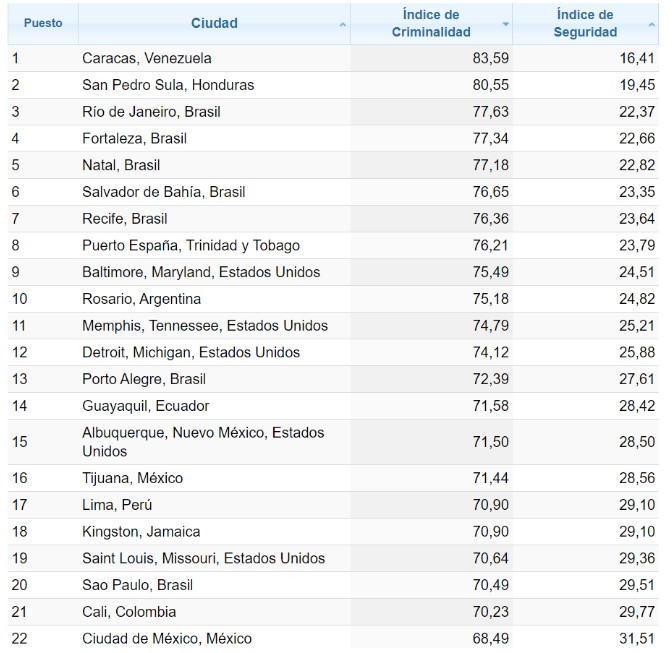
\includegraphics[width=0.65\textwidth]{1/figures/fig11.jpg}
		\caption{Índice de criminalidad de los países de América 2023}
		\label{1:fig}
	\end{center}
\end{figure}

Según datos recopilados en la plataforma de Statista entre Julio y diciembre del 2023, por cada 100 habitantes en las zonas urbanas de Perú, el 11.9\% de esta población ha sido víctimas por el robo de pertenencias personales, como dinero, carteras o celulares, siendo esta, la más representativa y la que refleja la parte vulnerable de los ciudadanos al no hacer frente a los robos que se cometen en las calles. Si se toma en cuenta el tipo de acto delictivo que puede atentar a la vida humana en las calles, se tiene que, el robo de vehículos representa un 2\%, mientras que el secuestro y extorsión el 0.2\%; que, si bien son menos frecuentes, representan una amenaza al bienestar y seguridad de los ciudadanos de las zonas urbanas (Statista Research Department, 2024). El último informe del Organismo Supervisor de Inversión Privada en Telecomunicaciones (Osiptel) de 2023, se registraron un total de 1,706,643 casos de robo de celulares en el año 2023, el cual el mayor número de robo ha sido los días lunes (Infobae, 2024). Asimismo, se informó que, entre el periodo de enero y mayo del año 2023, por cada hora, se roban en promedio, 200 celulares a nivel nacional (El Comercio, 2023). Estos resultados no solo representan una pérdida material y económica por parte de los afectados, genera desconfianza y preocupación sobre su seguridad personal y la posible vulneración en su privacidad de información que se contenía en el dispositivo del agraviado.
 %\medskip
\begin{figure}[h]
	\begin{center}
		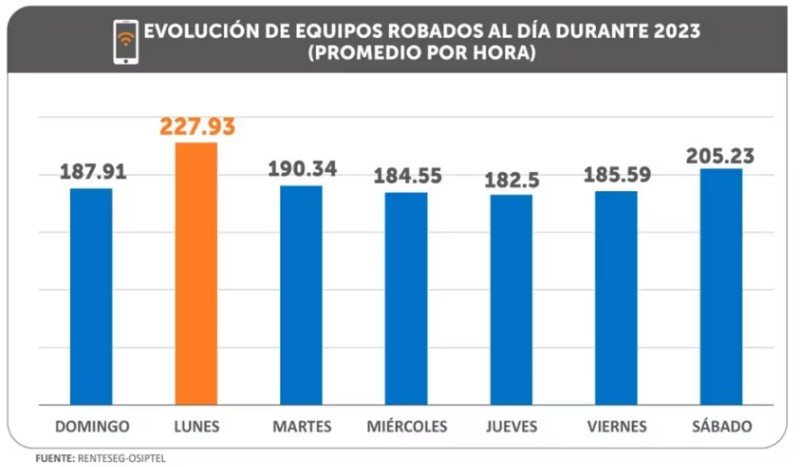
\includegraphics[width=0.65\textwidth]{1/figures/fig1.jpg}
		\caption{Días con más robos de celulares registrados en el 2023 Osiptel}
		\label{1:fig2}
	\end{center}
\end{figure}


Con lo que respecta al robo de vehículos, que también atenta a la vida y seguridad de la población de las zonas urbanas, según la Asociación Automotriz del Perú (APP) en el año 2023, la venta de vehículos ha representado un aumento del 2.4\% (181,000 autos vendidos) con respecto al año 2022 (AmChamnews, 2024). Este incremento en la venta de autos, también lleva consigo el aumento a los robos de vehículos, que es un problema que se está volviendo cada vez más persistente en Perú, ya que, según la Superintendencia Nacional de Registros Públicos, en promedio se roban 46 autos al día y que en el primer semestre del año 2022 se ha registrado un total de 9,758 autos robados en el Perú (Tracklink, 2023). 

Estas cifras demuestran la necesidad de desarrollar herramientas y/o estrategias que permitan mitigar los riesgos relacionados con los actos delictivos en entornos rurales, donde se destaca el robo de celulares y vehículos, que, a su vez, pueden estar relacionadas entre sí. Las aplicaciones móviles para ayudar al usuario a elegir rutas más cortas para llegar a su destino en el menor tiempo posible mediante un motor de crowdsourcing (recopilación de tráficos), son cada vez más comunes y fundamentales de utilizar; ya que, en 2022, más de 150 millones de personas utilizan Waze; mientras que Google maps ha sido instalada por más de 10 mil millones de usuarios (autocosmos, 2022). Sin embargo, estas herramientas de ayuda no tienen una funcionalidad que les permita detectar entre qué calles son seguras o no tomando en cuenta información o denuncias de delitos cometidos en esas zonas, ocasionando que los usuarios queden expuestos a situaciones peligrosas como el robo de su celular, de su auto o ambas. 



\section{Formulación del Problema}

Para lefecto \parencite{ot_marti2018manual}. 


Una vez elaborado el diagrama (véase Anexo 1), 

\subsection{Problema General}
\newcommand{\ProblemaGeneral}{
	¿Es posible utilizar un algoritmo de aprendizaje profundo para detectar rutas seguras en las calles de los Ángeles? 
}
\ProblemaGeneral
\subsection{Problemas Espec\'{i}ficos}
\newcommand{\Pbone}{
¿Qué algoritmos de aprendizaje profundo son los más representativos de los antecedentes?
}
\newcommand{\Pbtwo}{
¿Qué alternativas de procesamiento de datos se deben aplicar a la base de datos para entrenar el modelo?
}
\newcommand{\Pbthree}{
¿Qué métricas propuestas en los antecedentes existen para ayudar en la eficiencia y eficacia del modelo propuesto?
}
\newcommand{\Pbfour}{
¿El modelo propuesto evita las zonas con alto nivel de delincuencia?
}

\begin{itemize}
	\item \Pbone
	\item \Pbtwo
	\item \Pbthree
	\item \Pbfour
\end{itemize}

\section{Objetivos de la Investigación}
Para la formulación de los objetivos de la presente investigación se elaboró un «árbol de objetivos» (véase Anexo 2) 
\subsection{Objetivo General}
\newcommand{\ObjetivoGeneral}{
Desarrollar un algoritmo de aprendizaje profundo para detectar rutas seguras en las calles de los Ángeles.
}
\ObjetivoGeneral
\subsection{Objetivos Espec\'{i}ficos}
\newcommand{\Objone}{
Seleccionar los algoritmos de aprendizaje profundo más representativos de cada antecedente para la detección de rutas seguras.
}
\newcommand{\Objtwo}{
Seleccionar una alternativa de procesamiento de datos que permita entrenar un modelo de detección de rutas seguras.
}
\newcommand{\Objthree}{
Evalular la factibilidad del modelo con las métricas propuestas en los antecedentes para mejorar el tiempo de procesamiento con los menores recursos.
}
\newcommand{\Objfour}{
Demostrar que el modelo propuesto evita las zonas con alto nivel de delincuencia.
}

\begin{itemize}
	\item {\Objone}
	\item {\Objtwo}
	\item {\Objthree}
	\item {\Objfour}
\end{itemize}

\section{Justificación de la Investigación}

\subsection{Teórica}
Esta investigación se realiza 

\subsection{Práctica}
Al culminar la investigación 

\subsection{Metodológica}. 

\section{Delimitación del Estudio}

\subsection{Espacial}
Para la presente investigación se realizará con los registros de actos delictivos recolectados y almacenados en la web oficial del Departamento de Policía de los Ángeles (APD) para uso público, la cual consiste en denuncias o actos registrados por personas, junto con el tipo de delincuencia y la dirección dónde ocurrió el hecho. Estos datos están registrados en formato “csv”. Además, se utilizará librerías que permitan cartografiar las calles de la ciudad de los Ángeles y poder utilizarlos como grafos.
\subsection{Temporal}
La presente investigación analizará un conjunto de datos de registros delictivos de la ya mencionada base de la web oficial del APD, que empieza desde el año 2020 hasta los últimos registros descargados a la fecha que se inicia este trabajo.

\subsection{Conceptual}
Esta investigación se centrará en el desarrollo de un algoritmo que logre detectar qué rutas de la ciudad de los Ángeles serán seguras para evitar algún caso de crimen basado en un indicador de riesgo. Para lograrlo, se necesitará herramientas de Aprendizaje Profundo y métodos de procesamiento de datos para desarrollar un modelo que se adapte a los diferentes estilos de grafos de forma óptima. El modelo desarrollado busca poder dar una contribución a la comunidad con el fin de evitar situaciones peligrosas y apoyar a los distintos métodos de reducción en la tasa de criminalidad que se presenta en las zonas urbanas; asimismo aumentar la participación en técnicas de Aprendizaje Profundo utilizando grafos. 

\section{Hipótesis}

\subsection{Hipótesis General}
\newcommand{\HipotesisGeneral}{
Mediante el desarrollo de un algoritmo de aprendizaje profundo se logra detectar rutas seguras en las calles de los Ángeles.
}
\HipotesisGeneral
\subsection{Hipótesis Específicas}
\newcommand{\Hone}{
La selección de los algoritmos de aprendizaje profundo más representativos de cada antecedente mejora significativamente la precisión y eficiencia al detectar rutas seguras.
}
\newcommand{\Htwo}{
La identificación de una alternativa de procesamiento de datos influye positivamente para poder entrenar un modelo de detección de rutas seguras.
}
\newcommand{\Hthree}{
La utilización de métricas propuestas en los antecedentes es factible para optimizar el tiempo de procesamiento del modelo.	
}
\newcommand{\Hfour}{
Se demuestra que el modelo propuesto evita las zonas con alto nivel de delincuencia.
}
\begin{itemize}
	\item \Hone
	\item \Htwo
	\item \Hthree
	\item \Hfour
\end{itemize}

\subsection{Matriz de Consistencia}
A continuación se presenta la matriz de consistencia elaborada para la presente investigación (véase Anexo \ref{1:table}).


\chapter{MARCO TEÓRICO}
\section{Antecedentes de la investigación}
En esta sección se presentarán diversos artículos de investigación o tesis las cuales abordarán diversas técnicas y enfoques que se emplearon para afrontar problemas similares al de esta tesis. Asimismo, a continuación se presenta un cuadro resumen (véase Anexo \ref{A:table}) de lo que se presenta en esta sección.


\subsection{Real-time deep reinforcement learning based vehicle navigation \citep*{pr_dehghani2018copper}}
\citeauthor{pr_dehghani2018copper} realizaron un artículo de investigación el cual fue publicado en la revista «Applied Soft Computing» en el año 2020. Este fue titulado \citetitle{pr_dehghani2018copper} la cual traducida al español significa «Navegación de vehículos basada en aprendizaje de refuerzo profundo en tiempo real».

\subsubsection{Planteamiento del Problema y objetivo }
Los autores del siguiente artículo mencionan la gravedad del problema de la congestión vehícular en las ciudades contemporáneas, teniendo como consecuencia el alto consumo innecesario de energía, la contaminación y el tiempo invertido en viaje. Además, menciona la dificultad que tienen los algoritmos existentes para la optimización de las carreteras con el fin de afrontar dicho problema, siendo esta la complejidad que tienen los vehículos al interactuar en un entorno dinámico en tiempo real. Por lo que el objetivo de los autores es implementar un modelo de aprendizaje por refuerzo profundo (DRL) con el fin de construir un sistema de navegación en tiempo real a través de una secuencia de decisiones.

\subsubsection{Metodología empleada por los autores}
Este artículo propone un framework el cual primero construye una simulación en SUMO, que contiene una interfaz de Control de Tráfico (TraCI) y que utiliza mapas urbanos reales en OpenStreetMap mediante el método NETCONVERT. Luego en la misma simulación de SUMO, se puede extraer y pre procesar los datos a través del método TraCI que recupera el número de vehículos, el tiempo de viaje esperado, y la posición actual y el destino.

La segunda parte del framework propuesto es el middleware, que conecta el entorno de SUMO con las redes neuronales DRL bajo un método mejorado de Deep Q-Learning Network (DQN) para mantener y actualizar las políticas de navegación y proporciona comandos para la navegación. El modelo propuesto contiene un esquema de exploración de dos etapas que buscan mejorar la convergencia de la red así como su velocidad. La primera etapa se utiliza la política convencional y la segunda etapa es un método basado en la distancia para reemplazar la selección de una ruta. La estructura de la red neuronal profunda contiene 5 capas conectadas, la primera capa de entrada contiene 150 neuronas, las dos capas ocultas tienen 100 neuronas bajo la función de activación RELU, una estructura de duelo y su capa de salida. %\medskip

\begin{figure}[h]
	\begin{center}
		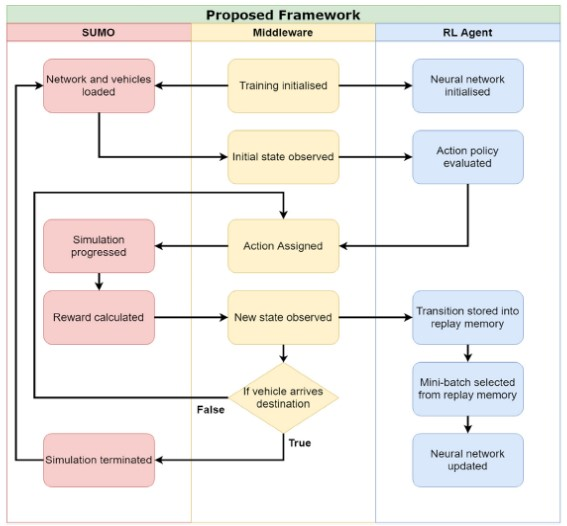
\includegraphics[width=0.65\textwidth]{2/figures/SUMO.jpg}
		\caption{Framework propuesto}
		\label{1:fig2}
	\end{center}
\end{figure}
%%%Ecuacion
%\begin{equation}  
%\label{eq:RMSE}
%RMSE = \sqrt{\frac{\sum_{i=1}^{N}{\Big(O_i -T_i\Big)^2}}{N}}
%\end{equation}

\subsubsection{Resultados obtenidos}
Para demostrar la eficiencia del modelo propuesto, se compara con diferentes modelos por ciudad, los resultados de una ciudad demuestran que el modelo reduce como máximo el tiempo de viaje en 5.3\%, 5.1\% y 16.4\% dependiendo de la demanda del tráfico. Otro indicador que se utiliza para medir su eficacia es la prueba de Wilcoxon, demostrando que el modelo propuesto es superior a los demás modelos.%\medskip

\begin{figure}[h]
	\begin{center}
		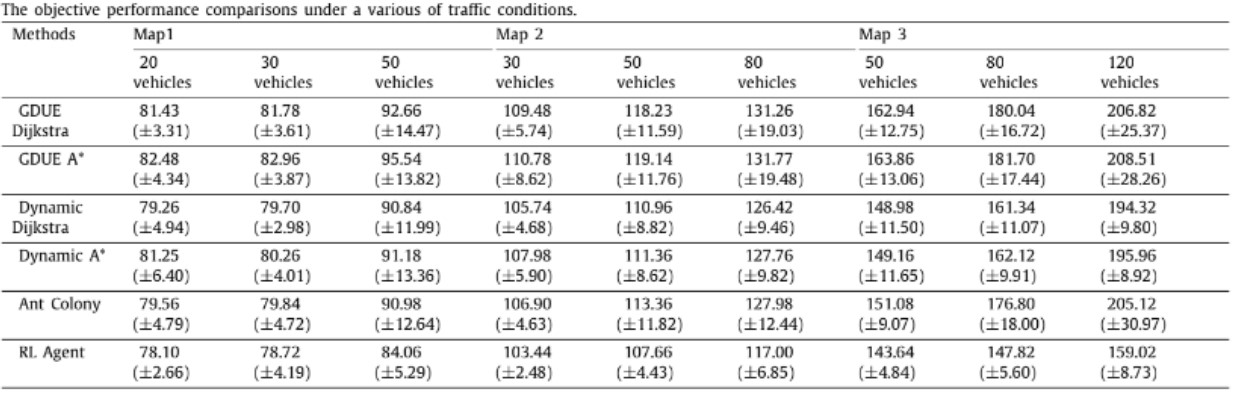
\includegraphics[width=0.65\textwidth]{2/figures/ResultSumo.jpg}
		\caption{Comparación de rendimiento de los modelos}
		\label{1:fig2}
	\end{center}
\end{figure}

%\medskip

 \begin{figure}[h]
	\begin{center}
		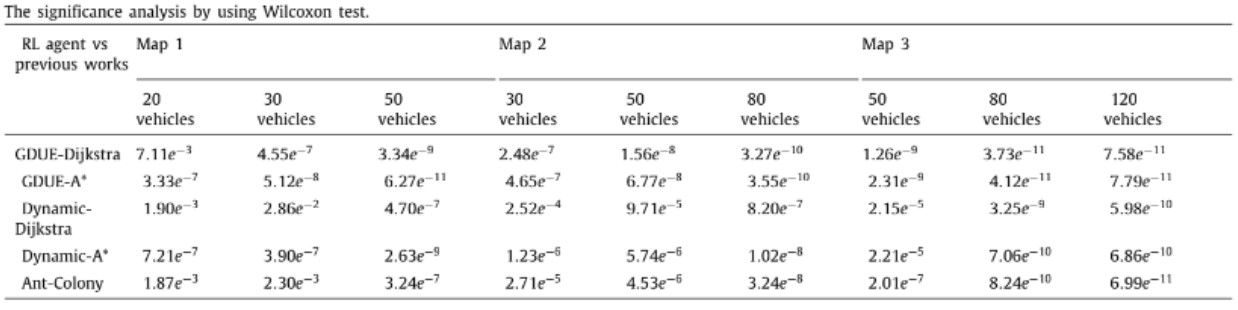
\includegraphics[width=0.65\textwidth]{2/figures/Result2Sumo.jpg}
		\caption{Análisis de significancia de los modelas con la prueba de Wilcoxon}
		\label{1:fig2}
	\end{center}
\end{figure}

\subsection{SafeRoute: Learning to navigate streets safely in an urban environment \citep*{pr_dehghani2018copper}}
\citeauthor{pr_dehghani2018copper} realizaron un artículo de investigación el cual fue publicado en la revista «ACM Transactions on Intelligent Systems and Technology» en el año 2020. Este fue titulado \citetitle{pr_dehghani2018copper} la cual traducida al español significa «SafeRoute: aprender a navegar por las calles de forma segura en un entorno urbano».

\subsubsection{Planteamiento del Problema y objetivo }
Ante los resultados de estudios realizados en la Universidad de Cornell y Hollaback en 2014, se muestra que el 85\% de mujeres tomaron rutas diferentes para ir a su destino con el fin de evitar ser víctimas de acoso o agresión. También se menciona la necesidad de las personas, como los turistas, de contar con una aplicación que pueda detectar rutas seguras. Con esto en mente, se propone SafeRoute, que es una solución de estos problemas utilizando algoritmos de aprendizaje por refuerzo profundo, que tiene ventaja bajo los algoritmos clásicos como Dijkstra, ya que es una opción a problemas que requieren tomar decisiones incrementales por cada intersección que se presenta entre el origen y el destino, además que tiene la ventaja de adaptarse a nuevos datos sin requerir a ser entrenado nuevamente.


\subsubsection{Metodología empleada por los autores}
Se emplea información pública de delitos de la ciudad de Nueva York, San Francisco y Boston, y se filtra los tipos de delitos relacionados con acoso callejero y asalto, los cuales son tiroteo, asalto y robo. Asimismo, para la obtención cartográfica de dichas ciudades, se utilizó OpenStreetMap (OSM).
%\medskip

\begin{figure}[h]
	\begin{center}
		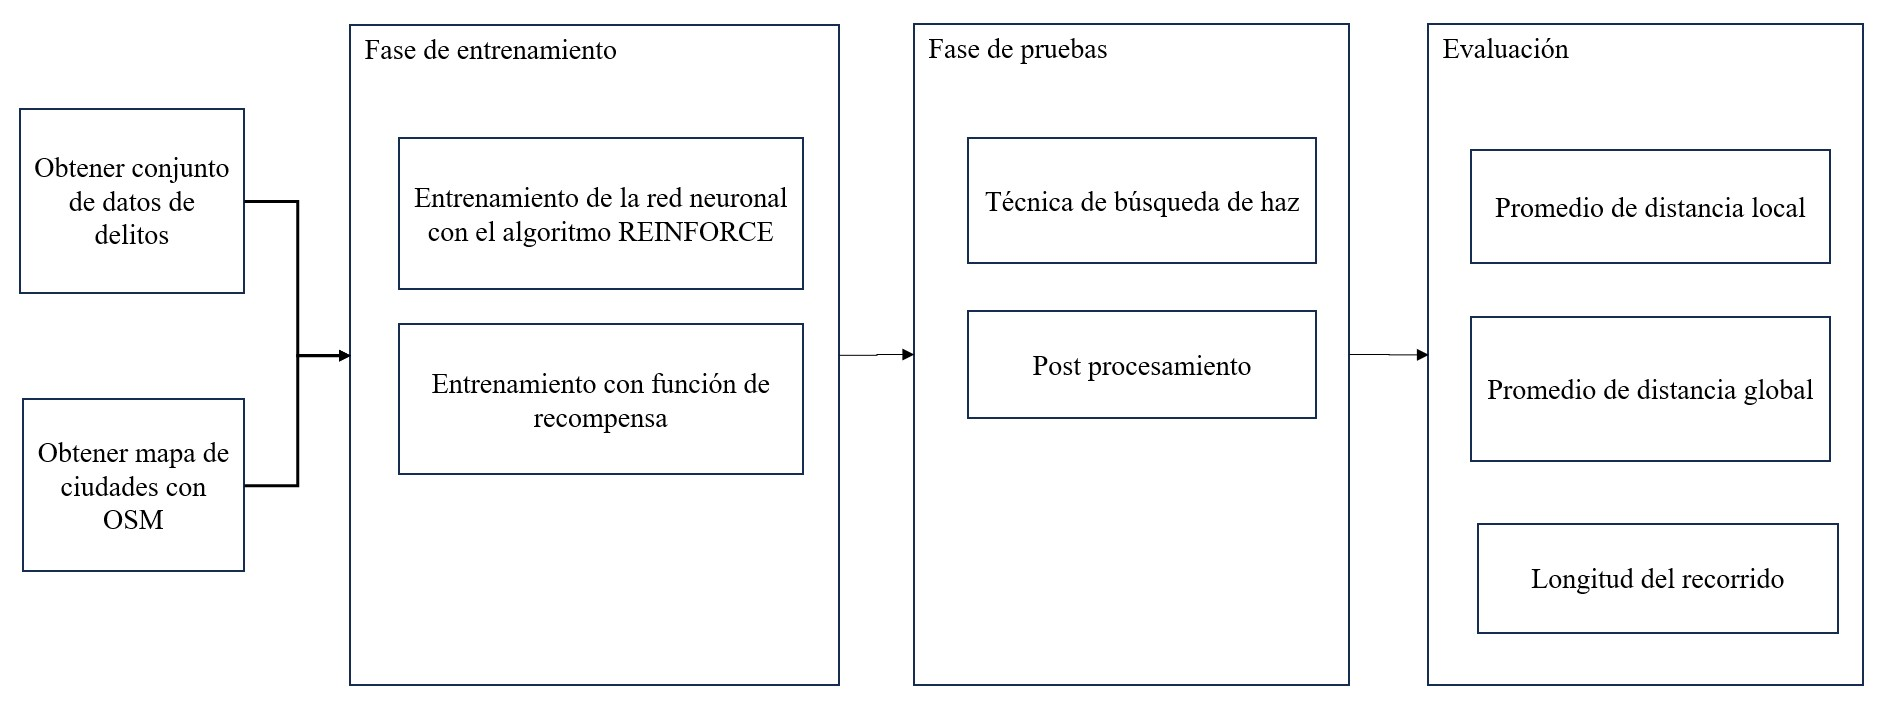
\includegraphics[width=0.65\textwidth]{2/figures/SafeMetodo.jpg}
		\caption{Metodología propuesta por los autores}
		\label{1:fig2}
	\end{center}
\end{figure}

De acuerdo a la metodología propuesta por los autores, la arquitectura se divide en dos partes, la primera es donde interviene la red neuronal de aprendizaje por refuerzo, y el segundo es la red de políticas definidas para que la red neuronal utiliza al momento de tomar decisiones. Este entorno se presenta como proceso de decisión de Markov con tuplas que contienen los estados contínuos del mapa, las acciones disponibles para el algoritmo y la probabilidad de pasar de un estado a otro.
%\medskip

\begin{figure}[h]
	\begin{center}
		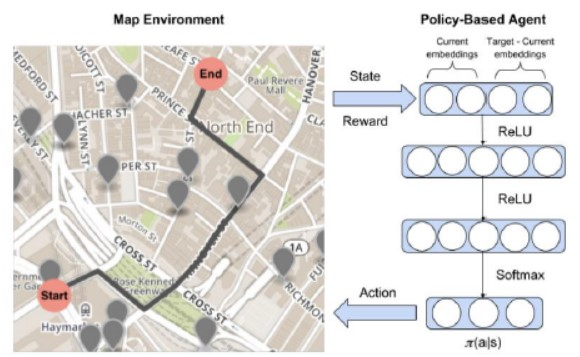
\includegraphics[width=0.65\textwidth]{2/figures/safeRouteAgent.jpg}
		\caption{Estructura de la red neuronal del modelo propuesto}
		\label{1:fig2}
	\end{center}
\end{figure}

Se establece una función de recompensa para optimizar las múltiples preferencias del modelo, en este caso es evitar las áreas de crimen al crear una ruta. La definición de esta función se establece de la siguiente manera:
%\medskip
\begin{figure}[h]
	\begin{center}
		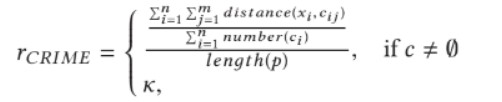
\includegraphics[width=0.65\textwidth]{2/figures/EcuacSafe.jpg}
	\end{center}
\end{figure}

Donde n es el número de bordes de cada camino, m es el número de delitos de cada nodo, x es la lista de puntos de cada camino, c es la lista de delitos de cada radio, p es el recorrido y k es un hiper parámetro.

En la fase de entrenamiento, consta de dos partes, la primera es el pre entrenamiento de la red neuronal para detectar rutas más cortas, en este proceso se utilizan técnicas de aprendizaje por refuerzo, específicamente el algoritmo Monte Carlo Policy Gradient (REINFORCE) para que actualice los parámetros de la red neuronal. La segunda es el entrenamiento con recompensas, donde se entrena nuevamente a la red neuronal considerando la seguridad en cada ruta, premiandolo por evitar áreas con alto índice de crimen, el cuál es la función de recompensa, y de esta manera actualizando la política de la red neuronal.

En la fase de pruebas, se utiliza una técnica de búsqueda de haz para encontrar varias rutas potenciales, luego se realiza un post procesamiento que evite bucles externos que se hayan creado durante la navegación, con el fin de que la ruta generada sea coherente y eficiente.
Para la evaluación del modelo propuesto con respecto a otros modelos, se aplicaron métricas cómo el promedio de la distancia local, el promedio de la distancia global y la longitud del recorrido. 

\subsubsection{Resultados obtenidos}
El modelo propuesto se comparó con el algoritmo de Dijkstra y SafePath, el cual crea produce caminos no dominados tomando en cuanto la seguridad. Se obtuvieron los mejores resultados con una tasa de aprendizaje de 0.0005 y realizando 5 saltos para un primer entrenamiento y luego 10 saltos. %\medskip

\begin{figure}[h]
	\begin{center}
		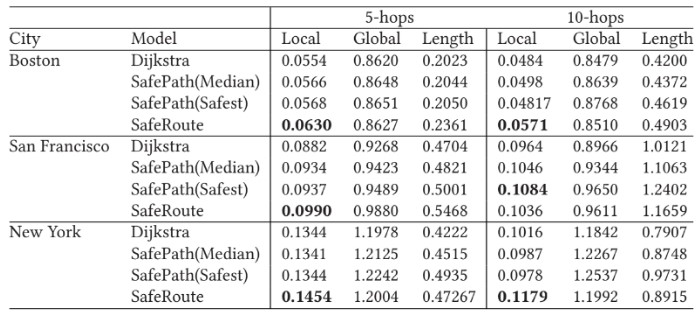
\includegraphics[width=0.65\textwidth]{2/figures/resultSafe.jpg}
		\caption{Comparación de rendimiento de los modelos}
		\label{1:fig2}
	\end{center}
\end{figure}

Se observa que las distancias entre un ruta a la zona de crimen, el que presenta un valor más bajo es Boston, debido a su densidad de criminalidad, mientras que las rutas generadas en Nueva York son las que más se alejan. Sin embargo, se demuestra que tanto en la época 5 como la época 10, el modelo propuesto SafeRoute supera al modelo Dijkstra y los modelos de SafePath, a excepción de la ciudad de San Francisco, el cuál el número que más se aleja de los riesgos es el modelo más seguro de SafePath en la época 10.

\subsection{Predicting motor vehicle theft in Santiago de Chile using graph-convolutional LSTM \citep*{pr_dehghani2018copper}}
\citeauthor{pr_dehghani2018copper} realizaron un artículo de investigación el cual fue presentado en la «39th International Conference of the Chilean Computer Science Society» en el año 2020. Este fue titulado \citetitle{pr_dehghani2018copper} la cual traducida al español significa «Predicción del robo de vehículos de motor en Santiago de Chile utilizando LSTM gráfico convolucional».

\subsubsection{Planteamiento del Problema y objetivo }
Ante el problema del incremento de autos robados en Chile en el año 2017, se menciona que este tipo de delitos, que, si bien es de bajo riesgo, puede desencadenar otros delitos más graves como el contrabando de armas o drogas, o crímenes internacionales. Es por esto que a través de un modelo de predicción de robo de vehículos puede contribuir a la mitigación y mayor seguridad por parte de la fuerza policial en las zonas con mayor probabilidad de robos. En este trabajo de investigación busca crear una nueva metodología para la predicción de robos de vehículos en la ciudad de Santiago de Chile desarrollando una red neuronal convolucional LSTM basada en grafos (GCLSTM) utilizando la técnica de preprocesamiento de datos, la cuál es la regresión LOESS.


\subsubsection{Metodología empleada por los autores}
Los autores proponen la siguiente metodología: %\medskip


\begin{figure}[h]
	\begin{center}
		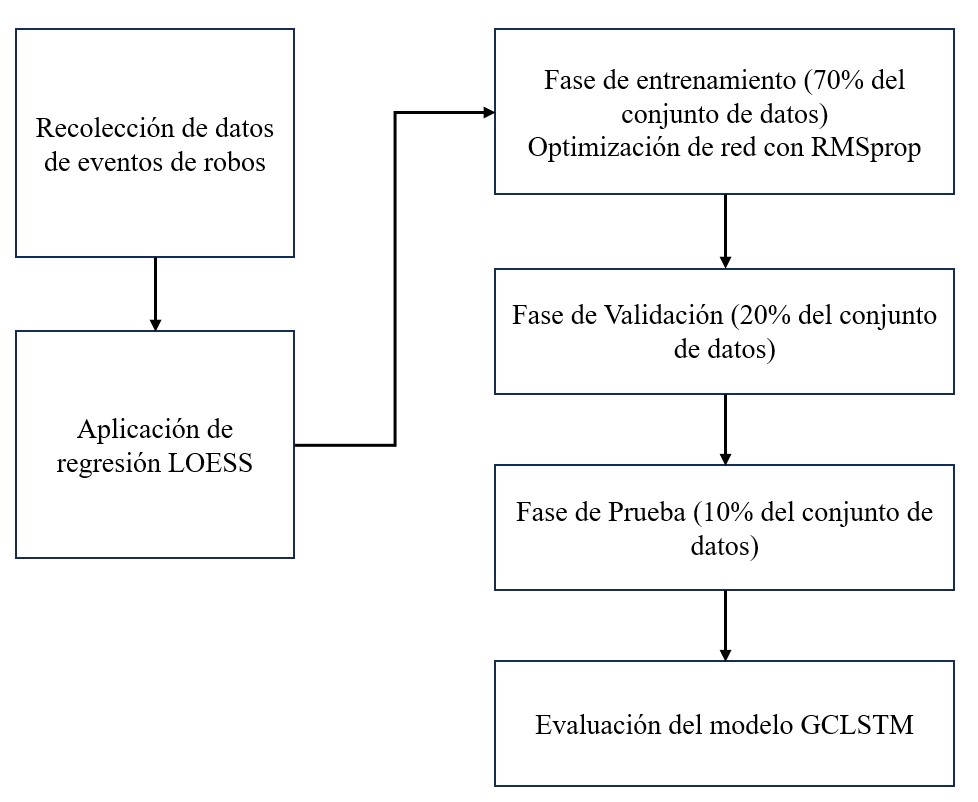
\includegraphics[width=0.65\textwidth]{2/figures/ChileMetodo.jpg}
		\caption{Metodología propuesta por los autores}
		\label{1:fig2}
	\end{center}
\end{figure}

El primer paso de esta metodología empieza con la recolección de los datos, que en este caso son los eventos de robos de vehículos en las comunas de la Región de Chile del año 2015 al 2019, que contiene un total de 129.127 registros. Luego se procedió a realizar la suma de los eventos de robo por día de cada comuna para la creación de una serie de tiempo y posterior a esto, aplicar la regresión LOESS, el cual es una técnica no paramétrica que utiliza los mínimos cuadrados ponderados para asignar un mayor peso a los más cercanos y menos a los que están más lejos. La aplicación de dicha técnica permite la reducción de ruido de la serie de tiempo. De este paso, se obtuvo una matriz suavizada de número de eventos de robos, el cuál sirve como input para la red GCLSTM. 

Dicha red suma las matrices de adyacencia e identidad para realizar la convolución con parámetros K, luego se le asigna a cada vecino un peso por iteración y estas van a las compuertas LSTM para la extracción de la última celda para el desarrollo de una capa de salida lineal con la función tanh. Para la optimización de la red GCLSTM, se aplicó el algoritmo de RMSprop para entrenar el modelo hasta que haya un sobreajuste en los datos.

%\medskip

\begin{figure}[h]
	\begin{center}
		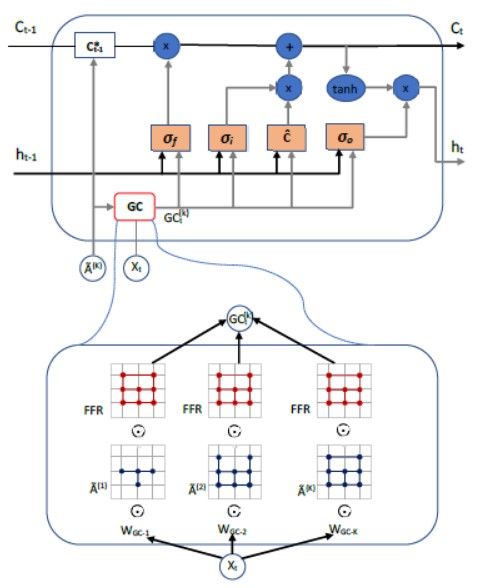
\includegraphics[width=0.65\textwidth]{2/figures/EsquivelRed.jpg}
		\caption{Estructura de la red convolucional LSTM basada en grafos}
		\label{1:fig2}
	\end{center}
\end{figure}

Para la fase de entrenamiento, se utilizó el 70\% del conjunto de datos, 20\% de validación y 10\% para la fase de prueba.

\subsubsection{Resultados obtenidos}
Como parte de los resultados, en la fase de entrenamiento, se entrenó en el modelo tradicional LSTM y el modelo GCLSTM, dando como resultado que a partir de la iteración 31, la curva MSE del modelo GCLSTM desciende más que el tradicional. 
Mientras que, en la fase de pruebas, se demuestra, con la métrica R2, que el modelo propuesto obtuvo 0.86, y el modelo LSTM tuvo 0.70, teniendo una mayor similitud la red GCLSTM entre lo esperado con lo observado. Por otra parte, el MSE del modelo propuesto fue 0.014 y el modelo LSTM es de 0.031; demostrando que el modelo puede obtener patrones temporales y espaciales para la predicción de crimen en distintas zonas de una ciudad. 

\subsection{Algoritmo para calcular la ruta más segura y óptima \citep*{pr_dehghani2018copper}}
\citeauthor{pr_dehghani2018copper} realizaron un artículo de investigación el cual fue publicado en el año 2022. Este fue titulado \citetitle{pr_dehghani2018copper}.

\subsubsection{Planteamiento del Problema y objetivo }
La creciente cifra de casos de acoso callejero en las calles de Medellín, así como casos de asaltos y violación, ha tenido como consecuencia que el miedo de las mujeres aumente y por ende, se sientan inseguras por cuál ruta tomar. A pesar de los distintos métodos de prevención, se menciona que no siempre son efectivos para evitar ser víctima de acoso en espacios públicos. Además, aplicaciones de generación de rutas para el transporte, como Google Maps o Waze, no cuentan con la capacidad de detectar rutas seguras, ya que es propio sistema de estas sólo calculan sus rutas en base a la distancia más corta. Este trabajo de investigación busca solucionar este problema implementando el algoritmo de Dijkstra, para calcular tres caminos diferentes tomando en cuenta la distancia y el índice de riesgo.

\subsubsection{Metodología empleada por los autores}
Para la obtención del mapa de Medellín, se empleó Open Street Maps (OSM) en Python, el cual contiene en cada segmento su longitud en metros, en qué sentidos va, y sus representaciones binarias proporcionadas por la propia librería OSM. Para el cálculo del riesgo, se empleó un conjunto de datos de la encuesta de calidad de vida de Medellín del año 2017; luego se procedió a realizar una combinación lineal (CL)  mediante el análisis de componentes principales, el cual  es la máxima varianza de la proporción de hogares que se sienten inseguros entre la proporción de hogares que tienen ingresos inferiores al salario mínimo; después se normaliza la combinación lineal y la proporción de esta es considera como el riesgo de acoso.
%\medskip

\begin{figure}[h]
	\begin{center}
		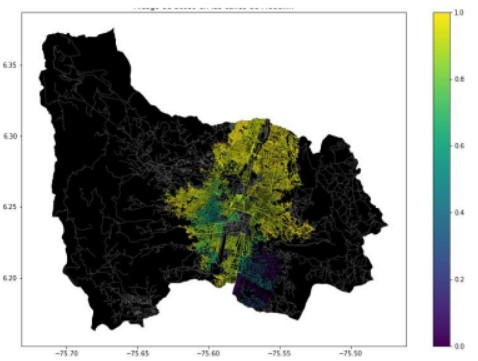
\includegraphics[width=0.65\textwidth]{2/figures/segmento.jpg}
		\caption{Riesgo de acoso sexual mediante combinación lineal}
		\label{1:fig2}
	\end{center}
\end{figure}

Se crea un diccionario que almacena el peso de cada vértice mediante el producto entre la longitud y riesgo de acoso de cada relación entre origen y destino. Se implementa el algoritmo de Dijkstra que requiere de tres parámetros los cuáles son los grafos creados, y los vértices de origen y destino. Este algoritmo calcula cada vecino del vértice actual a través de sus pesos que están almacenados en el diccionario para calcular el camino con menos peso. Además del cálculo tradicional que emplea, el cuál es r*d, donde r es el riesgo de acoso, y d es la distancia en metros, se calculó dos caminos más. El primero es la suma entre la distancia y el riesgo, mientras que el segundo eleva la distancia al riesgo de acoso. Para graficar estos tres resultados, se empleó la librería GmPlot, une el camino del origen y destino mediante las coordenadas ubicadas en Google maps, siendo más fácil de visualizar para el usuario.
%\medskip


\begin{figure}[h]
	\begin{center}
		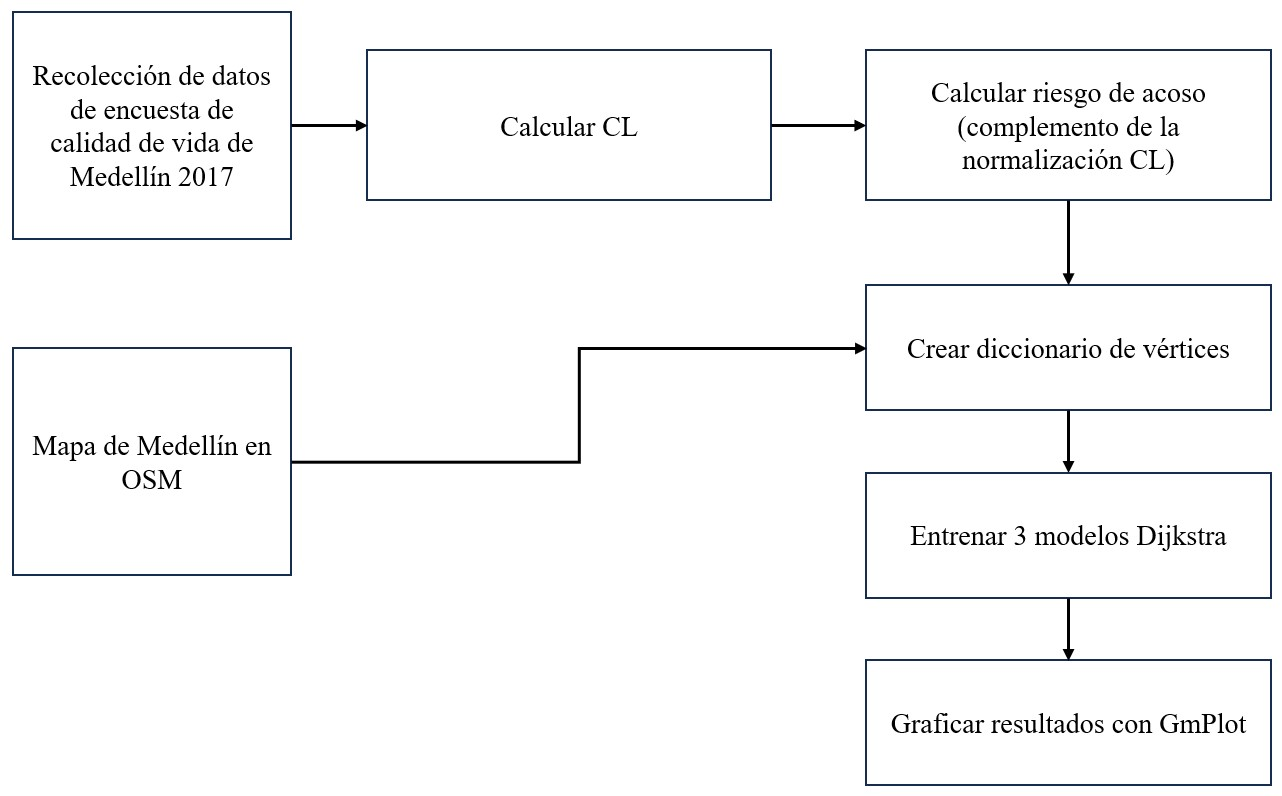
\includegraphics[width=0.65\textwidth]{2/figures/medellinMetodo.jpg}
		\caption{Metodología propuesta por los autores}
		\label{1:fig2}
	\end{center}
\end{figure}

\subsubsection{Resultados obtenidos}
Se presenta los resultados que son obtenidos por el algoritmo, estableciendo el origen en la Universidad EAFIT hasta la Universidad Nacional, el cual se puede visualizar en la siguiente tabla:%\medskip

\begin{table}[h]
	\centering
	\begin{tabular}{c|c|c|c}
		Camino & Distancia & Riesgo & Tiempo de ejecución\\\hline
		r*d & 9061.75m & 0.58& 1.01033s\\
		r+d & 8574m& 0.69& 1.01030s\\
		d\^r& 16642m& 0.35& 1.00640s
	\end{tabular}
	\caption{\label{tab:results}Tabla de resultados.}
\end{table}

%\medskip

Se observa que en términos de evitar el mayor riesgo, la mejor opción es el tercer camino (d\^r); sin embargo, la distancia que puede recorrer una persona es amplia a comparación de los otros caminos; asimismo, la opción más balanceada en cuanto al índice de riesgo y la distancia recorrida es el primer camino (r*d). También se demuestra que el tiempo de ejecución es bastante bajo, por lo que abre la oportunidad de ser empleado en una aplicación móvil para el fácil uso de los usuario que lo emplearán en su vida cotidiana.


%%%%%%%%%%%%%%%%%%%%%%%%%%%%%%%%%%%%%%%%%%%%%%%%%%%%%%%%%%
\subsection{Route-the safe: A robust model for safest route prediction using crime and accidental data \citep*{pr_dehghani2018copper}}
\citeauthor{pr_dehghani2018copper} realizaron un artículo de investigación el cual fue publicado la entrevista en el año 2019. Este fue titulado \citetitle{pr_dehghani2018copper} la cual traducida al español significa «Ruta segura: un modelo sólido para la predicción de rutas más seguras utilizando datos sobre delitos y accidentes».

\subsubsection{Planteamiento del Problema y objetivo }
La falta de conocimiento de la zona de una ciudad para un turista, así como invertir su tiempo en investigar sobre esta, puede crear una dependencia a sus conductores o pueden verse expuestas a ciertos peligros, como el robo de sus pertenencias. Asimismo, también se menciona la falta de capacidad que tienen las aplicaciones de rutas al momento de elegir un camino seguro. Con el objetivo de ser una herramienta de ayuda a la hora de elegir la ruta más segura para viajar, este proyecto  utiliza algoritmos de aprendizaje automático para la predicción de rutas seguras mediante el cálculo de puntuación de riesgo de cada ruta de las ciudad de Nueva York utilizando datos sobre delitos y accidentes.
\subsubsection{Metodología empleada por los autores}
Este trabajo de investigación presenta la siguiente metodología utilizada para la implementación de su modelo:
%\medskip

\begin{figure}[h]
	\begin{center}
		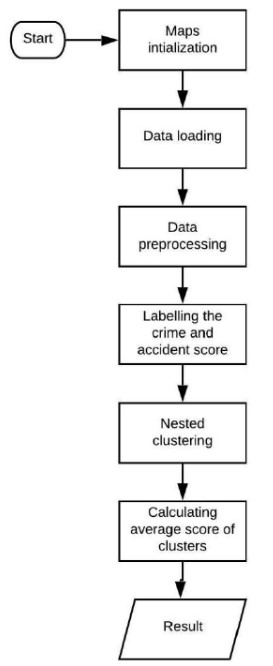
\includegraphics[width=0.35\textwidth]{2/figures/routeMet.jpg}
		\caption{Metodología Propuesta}
		\label{1:fig2}
	\end{center}
\end{figure}
%\medskip
Como primer paso de la metodología propuesta, se inicializa el mapa con el API de Google Maps, para luego proceder a configurar su función gmaps. Luego se cargan los datos, los cuáles contienen datos de delitos y accidentes desde el sitio web de datos abiertos de Nueva York, que brindan información del tipo de delito o accidente, así como su latitud y longitud. El siguiente paso se aplica al preprocesamiento de los datos para limpiar los datos atípicos o faltantes.
Una vez realizado el preprocesamiento de los datos, se procede a etiquetar la puntuación de accidentes de un punto (AS) y la puntuación de delitos de un punto (CS). Para la puntuación de delitos se asigna ponderaciones que van desde 1 a 15 dependiendo del delito y tipo de castigo que se le impone al sospechoso. Mientras que la puntuación de accidentes se calcula de la siguiente manera:

AS = PK*2 + CK*2 + MK*2 + PI + CI + MI

	Donde:

PK: Recuento de peatones fallecidos

CK: Recuento de ciclistas fallecidos

MK: Recuento de automovilistas fallecidos

PI: Recuento de peatones heridos

CI: Recuento de ciclistas heridos

MI: Recuento de automovilistas heridos

El siguiente paso es la formación de los grupos utilizando K Means, que es un algoritmo de agrupación de aprendizaje automático no supervisado, basado en la latitud y longitud, así como los conjuntos de datos se concatenan para agruparlos y determinar las regiones de riesgo. Específicamente, primero se agrupa en función a la longitud y latitud donde ocurrieron los hechos, para dividir el mapa de Nueva York en regiones más pequeñas. Asimismo, para generar las regiones de riesgo, se agrupa bajo los grupos ya formados en un distrito, como por ejemplo, el distrito de Manhattan. 

Después de hacer las agrupaciones de los grupos formados de un distrito, se realiza la puntuación promedio de cada agrupación, los cuáles se calculan de la siguiente manera:
%\medskip
\begin{figure}[h]
	\begin{center}
		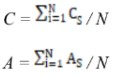
\includegraphics[width=0.25\textwidth]{2/figures/agrupSafe.jpg}
	\end{center}
\end{figure}
%\medskip
Donde N es el número de puntos de un grupo. Después se procede a calcular la puntuación del riesgo (RS) que toma como entrada el origen y destino de la ruta a calcular gracias al API de google maps llamado Direction Service,  que proporciona una serie de pasos al usuario para seguir la ruta. Luego se utiliza el modelo KNN Regresor para hallar el vecino más cercano según el grado de riesgo de cada punto. La puntuación de riesgo (RS) se calcula de la siguiente manera: 

%\medskip
\begin{figure}[h]
	\begin{center}
		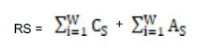
\includegraphics[width=0.25\textwidth]{2/figures/riesgoSafe.jpg}
	\end{center}
\end{figure}
%\medskip

Donde W es el número de puntos de rutas que hay entre el origen y el destino.

Como último punto, el modelo debe mostrar la ruta más segura bajo las siguientes dos condiciones: el primero es que la ruta debe presentar la puntuación de riesgo más baja, y la segunda es que si hay más de una ruta segura, se debe elegir la distancia más corta.
%\medskip
\begin{figure}[h]
	\begin{center}
		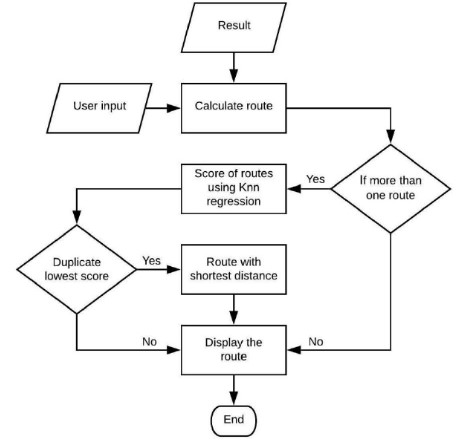
\includegraphics[width=0.35\textwidth]{2/figures/CondicionSafe.jpg}
		\caption{Flujo de condición para detectar rutas seguras}
		\label{1:fig2}
	\end{center}
\end{figure}
%\medskip

\subsubsection{Resultados obtenidos}
Se establece un punto de origen A y un punto de destino B en el distrito de Manhattan, dando como resultado que bajo el modelo de KNN Regressor, el R cuadrado de la puntuación de accidentes sea de 0.91 y la puntuación de criminalidad sea de 0.974; concluyendo que el modelo se ajusta mejor a sus datos.

%\medskip
\begin{figure}[h]
	\begin{center}
		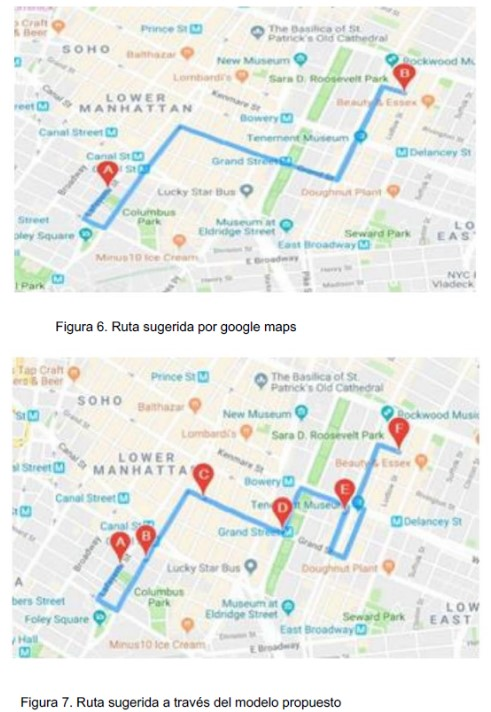
\includegraphics[width=0.4\textwidth]{2/figures/resultRoute.jpg}
		\caption{Resultados obtenidos}
		\label{1:fig2}
	\end{center}
\end{figure}
%\medskip

%%%%%%%%%%%%%%%%%%%%%%%%%%%%%%%%%%%%%%%%%%%%%%%%%%%%%%%%%%%%%%
%\medskip
\subsection{Real-time safest route identification: Examining the trade-off between safest and fastest routes \citep*{pr_dehghani2018copper}}
\citeauthor{pr_dehghani2018copper} realizaron un artículo de investigación el cual fue publicado en la revista «Analytic methods in accident research» en el año 2023. Este fue titulado \citetitle{pr_dehghani2018copper} la cual traducida al español significa «Identificación de la ruta más segura en tiempo real: examen de la relación entre las rutas más seguras y las más rápidas»..

\subsubsection{Planteamiento del Problema y objetivo }
Este trabajo de investigación propone un nuevo enfoque de predicción de rutas seguras debido a la creciente congestión vehícular y accidentes, esto con el fin de mejorar el flujo vehícular  de un determinado sector utilizando datos en tiempo real para que se sincronice con el modelo y proporcionar avisos para que el usuario evite regiones congestionadas o que están expuestos a peligros en las carreteras. Tiene como objetivo desarrollar un algoritmo de enrutamiento en tiempo real bajo una métrica propuesta que combina el riesgo de accidentes con el tiempo de viaje a lo largo de diferentes puntos de una ruta.

\subsubsection{Metodología empleada por los autores}
Se utiliza un conjunto de datos de código abierto llamado pNEUMA, de la ciudad de Atenas, Grecia. Este conjunto de datos utiliza drones para recopilar los datos sobre el tráfico en horas pico, asimismo, bajo esta recopilación, se extrae los datos de la posición, velocidad, aceleración y tipo de vehículo. Luego se pre procesaron los datos mediante la comparación por pares de trayectorias. Después se calculó el tiempo de coalición (TTC) de cada ubicación para aplicarlo al modelo propuesto.
%\medskip
\begin{figure}[h]
	\begin{center}
		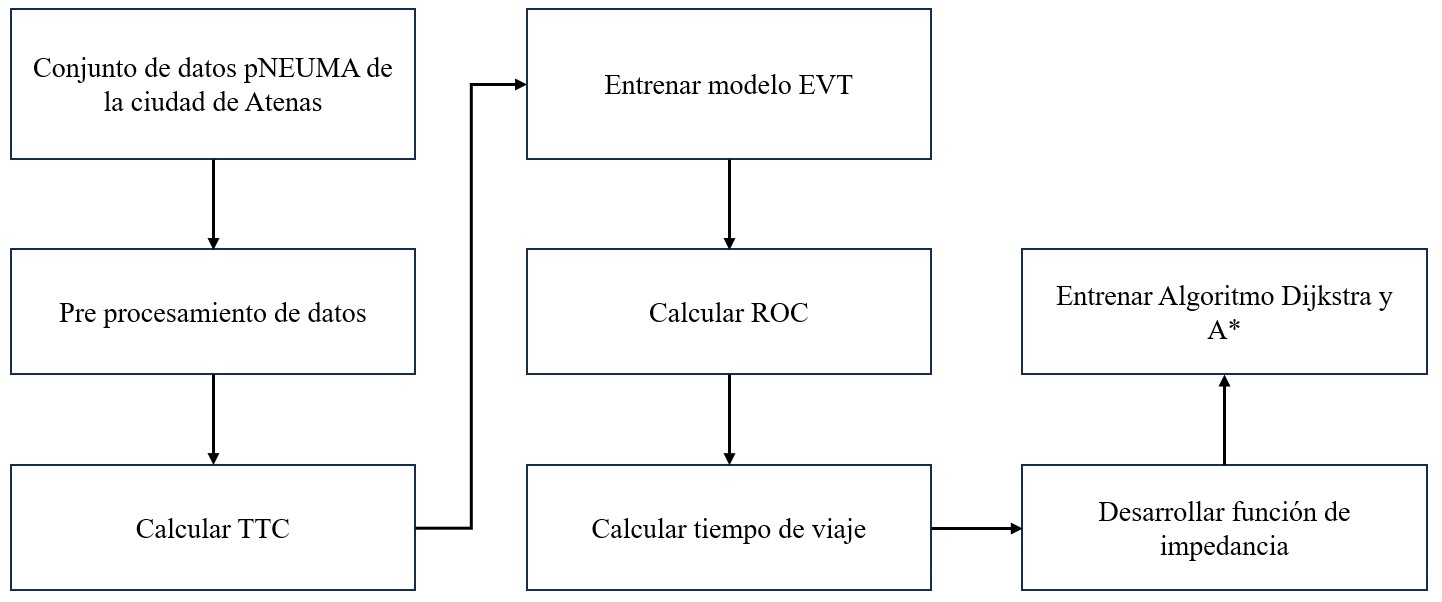
\includegraphics[width=0.65\textwidth]{2/figures/AtenaMetodo.jpg}
		\caption{Metodología propuesta por los autores}
		\label{1:fig2}
	\end{center}
\end{figure}
%\medskip

El modelo propuesto es un modelo de teoría de valores extremos (EVT), específicamente el modelo bayesiano jerárquico para estimar el riesgo de accidente de cada ubicación en tiempo real y se incorporan covariables para optimizar el rendimiento del modelo propuesto. Después de desarrollar el modelo bayesiano, se calcula el riesgo de colisión (ROC), que estima el número total de accidentes que se observan en una ubicación, también se calcula una métrica de tiempo de viaje para desarrollar una función de impedancia para realizar comparaciones entre los distintos nodos de una red de carreteras bajo un algoritmo de enrutamiento. Para el cálculo de la función de impedancia (S) es de la siguiente manera:

%\medskip
\begin{figure}[h]
	\begin{center}
		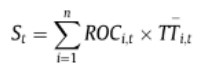
\includegraphics[width=0.35\textwidth]{2/figures/roc.jpg}
	\end{center}
\end{figure}
%\medskip

Posterior al cálculo de la función de impedancia, se utiliza en el algoritmo Dijkstra o el algoritmo A*. Después se desarrolla un algoritmo que elige la mejor ruta, el cuál identifica distintas rutas según la preferencia del usuario, tomando en cuenta tanto la seguridad como la movilidad.

\subsubsection{Resultados obtenidos}
Bajo la metodología propuesta, se encontró que el 23\% de las rutas más rápidas eran similares a las rutas más seguras. Además, la ruta más segura comparte en un 54\% los mismos enlaces que la ruta más rápida, existiendo un equilibrio entre seguridad y movilidad en distintos escenarios. Este trabajo de investigación aporta con un modelo de recomendación de rutas que presenta una buena eficacia en cuanto a cambios dinámicos en tiempo real en diferentes tipos de condiciones; sin embargo, para el cálculo de riesgo, depende de una percepción de seguridad más que la seguridad real, por lo que se recomienda que se establezca bajo su propia preferencia y prioridades, ya que es difícil cuantificar el riesgo real de un sector.

\subsection{A reinforcement learning-based routing algorithm for large street networks. \citep*{pr_dehghani2018copper}}
\citeauthor{pr_dehghani2018copper} realizaron un artículo de investigación el cual fue publicado en la « International Journal of Geographical Information Science» en el año 2024. Este fue titulado \citetitle{pr_dehghani2018copper} la cual traducida al español significa «Un algoritmo de enrutamiento basado en aprendizaje de refuerzo para grandes redes de calles».

\subsubsection{Planteamiento del Problema y objetivo }
Ante la problemática de contar con sistemas de evacuación y rutas de emergencia para minimizar los daños ocasionados durante los desastres naturales, los algoritmos tradicionales de enrutamiento cuentan con problemas de escalavidiad cuándo estas se enfrentan a evacuaciones a gran escala que involucran a diferentes rutas, asimismo, la complejidad computacional de estos algoritmos puede aumentar a medida que crece y se vuelve más complejo un escenario de evacuación, llevando a tener largos tiempos de cáculos, además que trabajan con pocos parámetros que capturan la complejidad y dinamismo de las emergencias por inundaciones. Ante estas limitaciones y con las contribuciones recientes de algoritmos de aprendizaje por refuerzo profundo (DRL), se desarrolló un algoritmo de aprendizaje por refuerzo para mejorar la eficiencia de enrutamiento en una gran red de carrenteras en tiempo real, para lograr dicho objetivo, se entrenó dicho algoritmo en una supercomputadora FASTER, que maneja grandes redes de carreteras de una base de datos espacial.

\subsubsection{Metodología empleada por los autores}
Se recopilan los datos de redes de transporte de la ciudad de Nueva York y Houston, que contienen la longitud y latitud de cada punto de interés, asimismo para los datos de transporte se exporta información cartográfica del área centra de Houston y la ciudad de Nueva York. 

Para el algoritmo de aprendizaje por refuerzo, el sistema de enrutamiento puede modelarse como una tupla de proceso de decisión de Markov (MDP. Cada tupla contiene el conjunto de estados de cada vértice, conjunto de acciones que considera la red neuronal durante el entrenamiento, la función de recompensa para optimizar la preferencia del usuario, donde se incorpora el factor de seguridad. Además, se establece políticas con el método de gradientes de políticas, el cual se conecta con el algoritmo de ascenso de gradiente estocástico. Para disminuir la varianza del estimado de gradientes del algorimo, se utiliza la Optimización de Política Proximal (PPO). 

%\medskip
\begin{figure}[h]
	\begin{center}
		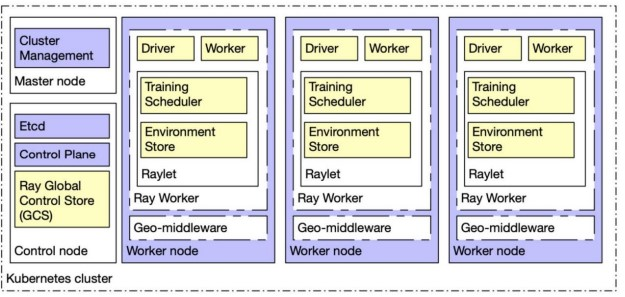
\includegraphics[width=0.65\textwidth]{2/figures/algoMod.jpg}
		\caption{Puntuaciones de evaluación}
		\label{1:fig2}
	\end{center}
\end{figure}
%\medskip

Para hacer frente a los entornos complejos y dinámicos, se requiere de una red neuronal que memorice los nodos y elija una acción válida a través de Q-learning, este algoritmo evita no seleccionar rutas inválidas con la red de políticas.

%\medskip
\begin{figure}[h]
	\begin{center}
		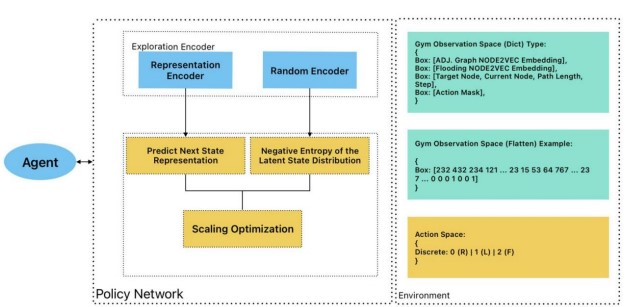
\includegraphics[width=0.65\textwidth]{2/figures/politica.jpg}
		\caption{Puntuaciones de evaluación}
		\label{1:fig2}
	\end{center}
\end{figure}
%\medskip

\subsubsection{Resultados obtenidos}
Se comparó con el método de Dijkstra y el algoritmo clásico de aprendiza por refuerzo mediante puntuación por métricas de seguridad y recompensa de cada ciudad, como también su tiempo. Los resultados indican que el mejor algoritmo es el modelo propuesto, ya que tienen un mayor puntaje de seguridad, como también un mayor indicador de recompensa. Sin embargo, tiene una mayor duración al ejecutar cada enrutamiento o detectar rutas seguras. También se destaca el hecho de que el modelo propuesto no atraviesa los puntos inundados, superando en términos de seguridad a los algoritmos tradicionales.

%\medskip
\begin{figure}[h]
	\begin{center}
		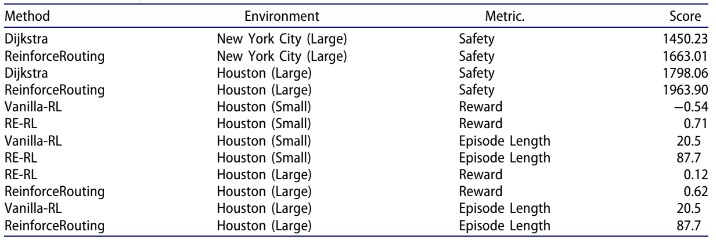
\includegraphics[width=0.65\textwidth]{2/figures/resultN.jpg}
		\caption{Puntuaciones de evaluación}
		\label{1:fig2}
	\end{center}
\end{figure}
%\medskip


\section{Bases Teóricas}
%\subsection{Machine Learning}
% Es un subcampo de l]ecutar dificultosos procesos aprendiendo de datos, en lugar de seguir reglas preprogramadas %\parencite{tec_royal2017machine}.

 %es importante mencionar que existen también cinco tipos de problemas de aprendizaje que se pueden enfrentar: regresión, clasificación, %simulación, optimización y clusterización \parencite{bk_gollapudi2016practical}. Por otro lado, el aprendizaje automático también posee una %división por subcampos que se puede observar en la Figura 14.
%%Figura
% \subsection{Natural Language Processing (NLP)}
 %Naturalmano \parencite{bk_goyal2018deep}. Otra definición para este término implica que es un campo especializado de la informática que es

 %De acuerdo con \citet{bk_goyal2018deep}, e
 
\subsection{Inteligencia Artificial}
La Inteligencia Artificial es el campo de la ciencia informática basada en máquinas que buscan replicar la inteligencia humana, implementando dotes como el razonamiento, aprendizaje y actuar que comúnmente podría hacer un humano \parencite{gl_DEFIA}. La Inteligencia Artificial va más allá que solo la comprensión, sino también el esfuerzo que conlleva construir entidades inteligentes; esto lleva a que su participación en la actualidad esté presente en una gran cantidad de campos, como el aprendizaje y la percepción, como también a campos más específicos como lo es el ajedrez \parencite{bk_russell2004intart}.
\subsubsection{Enfoques de Inteligencia Artificial \parencite{bk_russell2004intart}}
Russell también menciona que la definición de lo que es la Inteligencia Artificial sigue cuatro enfoques, en donde el sistema puede pensar y actuar de forma racional, como también de forma humana: 

\begin{itemize}
	\item \textbf{Actuar como humano:} Alan Turing sugiere una prueba llamada la Prueba de Turing el cual intenta demostrar las pocas diferencias que hay entre un agente inteligente y los seres humanos, ya que menciona que el computador necesita cumplir con seis disciplinas, las cuales son el procesamiento del lenguaje natural, la representación del conocimiento, un razonamiento automático que le permita extraer sus propias conclusiones y un aprendizaje automático que le pueda permitir adaptarse y detectar patrones; además, debe estar dotado con visión computacional y robótica.
	\item \textbf{Pensar como humano:} Considerado como el enfoque del modelo cognitivo, sugiere que el programa debe contar con un mecanismo necesario que le permita determinar cómo piensa un humano, por lo que es necesario penetrar el funcionamiento de dicha mente humana. Para lograr dicha penetración es a través de dos formas, la primera es capturando todos los pensamientos a medida que van apareciendo y la segunda es media una experimentación psicológica.
	\item \textbf{Actuar racionalmente:} Se espera que un agente racional actúe acorde al mejor resultado, o si en caso de que haya incertidumbre, elija la opción que proporcione el mejor resultado esperado. La Prueba de Turing puede permitir realizar dichas acciones racionales.
	\item \textbf{Pensar racionalmente:} Trata de construir sistemas inteligentes que sigan una lógica, el cuál es un esquema de estructuras de argumentación que le permita llegar a una conclusión correcta a partir de premisas correctas.
\end{itemize}
 
\subsection{Aprendizaje Automático}
El Aprendizaje Automático, o Machine Learning (ML) en inglés, forma parte de la rama de lo que es la Inteligencia Artificial, centrando su desarrollo en algoritmos y modelos capaces de  dotar a las computadoras con habilidades que mejoren el rendimiento de realizar una tarea específica sin requerir que sea programada \parencite{pr_diaz}. 

El Aprendizaje Automático utiliza algoritmos que puedan identificar patrones a través de datos almacenados y procesados para la creación de un modelo que le permita realizar análisis predictivos o de detección, ya que busca replicar la inteligencia humana para ser más precisos y mejoren a través de la práctica, siendo adaptable a cualquier escenario en donde los datos puedan cambiar \parencite{gl_azure}.

La aplicación del Aprendizaje Automático es muy amplia, como programas de motores de búsqueda, el diagnóstico automático médico, la detección de fraude en transacciones de una entidad bancaria, análisis de mercado y clasificación de objetos; además del uso de técnicas de reconocimiento facial, voz o escritura \parencite{pr_diaz}.

Existen tres métodos principales de Aprendizaje Automático:
\begin{itemize}
	\item \textbf{Aprendizaje Supervisado:} Se centra en el desarrollo de algoritmos donde interviene un programador para entrenar al modelo qué conclusiones debe hacer mediante un conjunto de datos etiquetados con un resultado ya definido \parencite{gl_oci}.  De esta manera, el modelo puede mapear las entradas con las salidas correctas, mediante una función de pérdida que mida la diferencia entre los verdaderos resultados con el resultado predicho del modelo \parencite{gl_super}. Este modelo puede resolver problemas de clasificación y de regresión, y está presente comúnmente en la detección de fraudes, enfermedades o la predicción del precio. 
	
	\item \textbf{Aprendizaje No Supervisado:} Presenta un enfoque más independiente, donde el modelo aprende a identificar patrones o procesos complejos sin la intervención constante de un programador. Dicho aprendizaje implica un entrenamiento mediante datos no etiquetados y sin un resultado esperado. Este aprendizaje utiliza algoritmos de agrupamiento como k-means, análisis de componentes principales o de asociación, también están en las técnicas de visión computacional. Estos algoritmos tienen como fin realizar grupos o agrupamientos de datos que comparten similitudes, como imágenes, las cuales cada grupo tiene su propia etiqueta \parencite{gl_oci}. 
	
	\item \textbf{Aprendizaje por Refuerzo:} El Aprendizaje por Refuerzo o Recompensa es la retroalimentación que se le da al agente para saber si algo bueno o malo ha ocurrido cuando realiza una acción. Este tipo de aprendizaje está presente en los juegos de ajedrez, donde el refuerzo se realiza cuando finaliza el juego \parencite{bk_russell2004intart}. El agente puede interactuar en un entorno dinámico, tomando decisiones y recibimiento retroalimentación mediante una función de recompensa, con el objetivo de aprender una política, el cual le brinda estrategias de selección para tomar acciones que maximicen el total de recompensas \parencite{gl_cordis}.
	%\medskip
	\begin{figure}[h]
		\begin{center}
			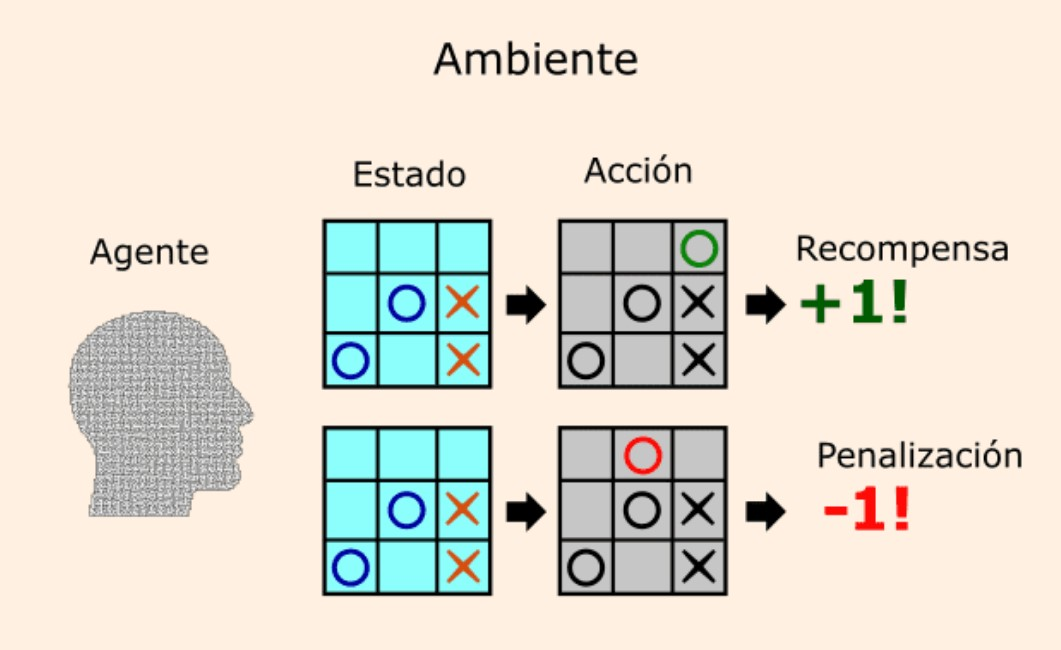
\includegraphics[width=0.65\textwidth]{2/MT/1.jpg}
			\caption{Representación del Aprendizaje por Refuerzo \\
				Fuente: \citep*{gl_ceupe}. \citetitle{gl_ceupe}}
			\label{1:fig2}
		\end{center}
	\end{figure}
	%\medskip
	
	Un concepto fundamental en la que se basa el Aprendizaje por Refuerzo es el Proceso de Decisión de Markov (MDP), el cuál es un marco matemático que le permite realizar un modelo de toma de decisiones en situaciones donde los resultados son aleatorios y depende del control de quien toma las decisiones. Como se muestra en la Figura \ref{1:mark},, este es un ejemplo simple de MDP, el cuál en cada paso de tiempo, el proceso inicia en un estado $S$, y el que toma la decisión puede elegir una acción a que está disponible en dicho estado. El resultado de esto otorga un nuevo estado $St$ y una recompensa $Ra (S, St)$ \parencite{gl_markov}.
	%\medskip
\begin{figure}[h]
	\begin{center}
		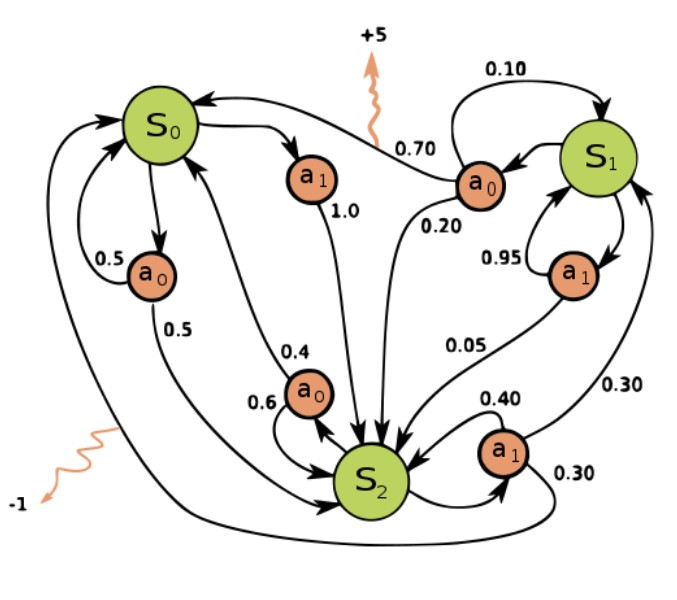
\includegraphics[width=0.65\textwidth]{2/MT/2.jpg}
		\caption{Proceso de decisión de Markov \\
			Fuente: \citep*{gl_markov}. \citetitle{gl_markov}}
		\label{1:mark}
	\end{center}
\end{figure}
%\medskip

Para que el MDP pueda conocer las probabilidades o dichas recompensas, se define una función el cuál es conocido como Q-learning:
%\medskip
\begin{equation} 
Q(s,a) = \sum_{s^{t}}P_{a}(s,s^{t})(R_{a}(s,s^{t})+\gamma V(s^{t}))
\end{equation}
%\medskip
Donde $P_{a}$ es la probabilidad de que la acción a en el estado $s$ en un tiempo determinado de un nuevo estado $s^{t}$, el $R_{a}$ es la recompensa esperada que recibirá de pasar un estado a otro debido a la acción $a$. Mientras que el $V$ contiene los valores reales del nuevo estado \parencite{gl_markov}.

\end{itemize}
\subsection{Aprendizaje Profundo}
Los algoritmos de aprendizaje profundo forman parte del aprendizaje automático, y los cuáles han tomado una mayor participación en los últimos años por la alta disponibilidad de grandes datos y los recursos computacionales potentes. Debido a que se cuenta con GPUs más rápidas para el entrenamiento de grandes modelos profundos, los algoritmos de Aprendizaje Profundo supera a los modelos tradicionales en múltiples aplicaciones, como el mejoramiento del rendimiento de modelos de reconocimiento de imágenes, redes neuronales convolucionales profundas al reducir la tasa de error, el rendimiento de sistemas de reconocimiento de voz el cual estuvo estancado varios años; y también aporta enormemente en el campo de la investigación del Procesamiento del Lenguaje Natural (NLP) \parencite{bk_grafo}.

\subsubsection{Redes Neuronales Profundas (DNN)}

Las Redes Neuronales Profundas, o Deep Neural Network en inglés, permiten al modelo mediante su entrenamiento a realizar tareas más complejas que son difíciles de hacer utilizando redes neuronales tradicionales. Asimismo, dichas redes se inspiran del cerebro humano, teniendo un diseño que no solo se limita a seguir reglas establecidas, sino también predecir y sacar conclusiones \parencite{gl_bot}. Las Redes Neuronales Profundas si bien son similares a las Redes Neuronales Tradicionales, el término de “Profundo” hace referencia al número de capas ocultas que forma parte de la red, teniendo más nodos de procesamiento, las cuáles son conocidas como neuronas \parencite{gl_edutech}.
    
%\medskip
\begin{figure}[h]
	\begin{center}
		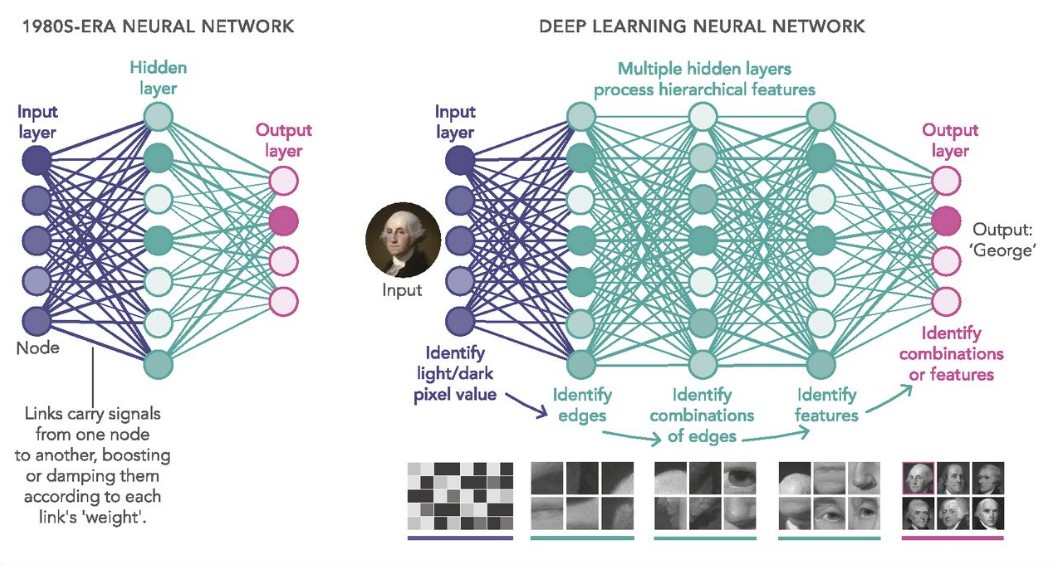
\includegraphics[width=0.65\textwidth]{2/MT/3.jpg}
		\caption{Comparación entre una Red Neuronal Artificial y una Red Neuronal Profunda \\
			Fuente: \citep*{gl_compara}. \citetitle{gl_compara}}
		\label{1:fig2}
	\end{center}
\end{figure}
%\medskip

Este tipo de red está presente en el reconocimiento de voz, sonidos y grafos, además que utilizan “Big Data” para la resolución de problemas en la que la intervención humana es limitada \parencite{gl_bot}. 


\subsection{Aprendizaje Profundo por Refuerzo (DRL)}
El Aprendizaje Profundo por Refuerzo o Deep Reinforcement Learning (DRL) es la combinación entre técnicas de Redes Neuronales Profundas con Aprendizaje por Refuerzo, esto tiene como beneficio la interacción de forma iterativa en un entorno para tomar decisiones que busquen maximizar una función de recompensas para encontrar estrategias más sofisticadas \parencite{gl_geekrein}. El Aprendizaje Profundo por Refuerzo es un paso importante en la evolución del aprendizaje de las máquinas que toma la decisión más beneficiosa y que utiliza esa decisión en escenarios futuros \parencite{gl_iic}.
%\medskip
\begin{figure}[h]
	\begin{center}
		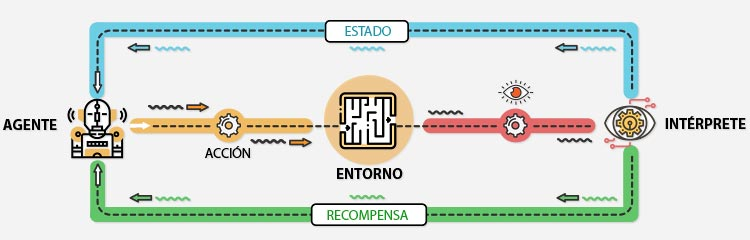
\includegraphics[width=0.65\textwidth]{2/MT/4.jpg}
		\caption{Componentes que conforma el Aprendizaje por Refuerzo \\
			Fuente: \citep*{gl_iic}. \citetitle{gl_iic}}
		\label{1:fig2}
	\end{center}
\end{figure}
%\medskip

 Un modelo de Aprendizaje Profundo por refuerzo está conformado por un agente, el cual es el que aprende las reglas a seguir y toma decisiones mediante la interacción con el entorno utilizando técnicas de Redes Neuronales Profundas.  Se menciona, además, que el DRL está basado en Q-learning, componentes de políticas para que se diriga las decisiones del agente, conceptos claves como lo son la función de valor que calcula las recompensas, las cuales son una señal que muestra el entorno sobre la acción deseada para que el agente cambie el estado de la situación actual del entorno. Son ampliamente utilizados en los sistemas de navegación, tratamientos médicos como la recomendación de medicamentes, perfeccionar los diseños de materiales con el fin de aumentar su efectividad y la personalización del entorno de eCommerce según los gustos de cada cliente \parencite{gl_iic}.
 
Con lo que respecta a los sistemas de navegación, se aplican tecnologías de información avanzadas para hacer frente al problema del control adaptativo de las señales de tráfico. Existen muchas investigaciones y propuestas como un enfoque que realiza simulaciones con datos de tráfico reales de la ciudad de Toronto, donde los agentes se coordinan mediante intersecciones vecinas. También la integración de un algoritmo de Aprendizaje por Refuerzo multiagente para enfrentar a los desafíos de estacionariedad y dimensionalidad en el control adaptativo de las señales de tráfico \parencite{pr_artiDeep}.

\subsubsection{Deep Q-Network (DQN)}
Para que el modelo de Aprendizaje Profundo por Refuerzo pueda aprender, es fundamental tener una función de valor. Esta función está presente en las arquitecturas DQN, la cuál nace en el año 2015 por DeepMind \parencite{pr_artiDeep}. Este algoritmo es creado por la necesidad de afrontar la inestabilidad de aprendizaje de la combinación de RL con redes neuronales, ya que almacena todo lo aprendido por el agente y luego lo reproduce aleatoriamente para proporcionar datos de entrenamiento diverso y des correlacionados \parencite{gl_DeepMind}. 

%\medskip
\begin{figure}[h]
	\begin{center}
		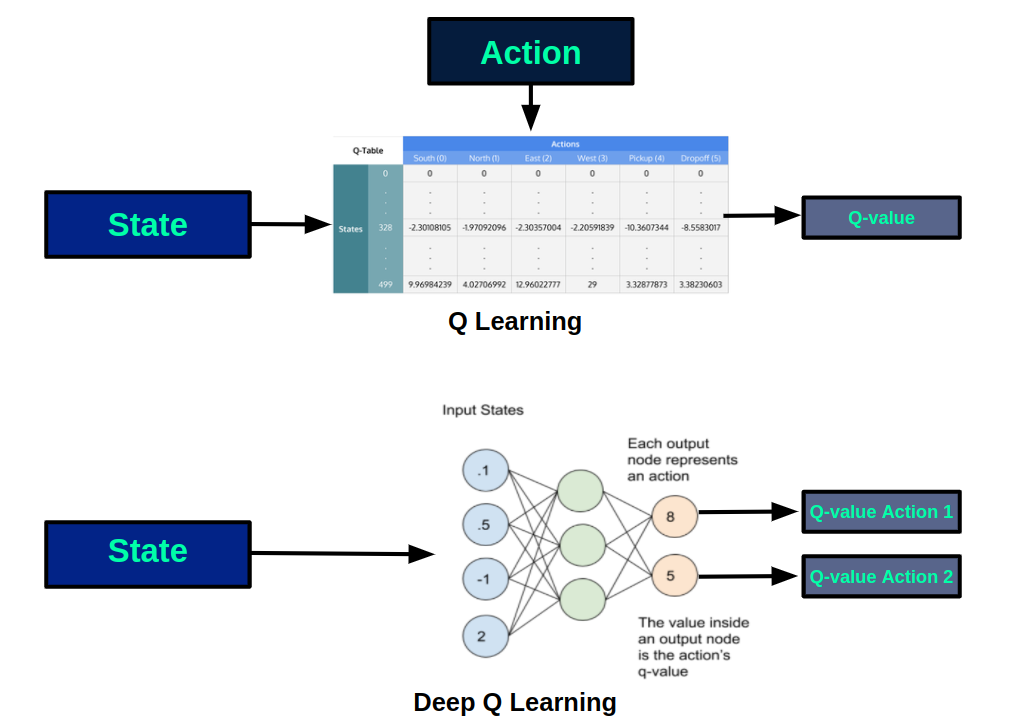
\includegraphics[width=0.65\textwidth]{2/MT/5.png}
		\caption{Diferencias entre Q-Learning y Deep Q-Learning \\
			Fuente: \citep*{gl_Damavis}. \citetitle{gl_Damavis}}
		\label{1:fig2}
	\end{center}
\end{figure}
%\medskip

Este algoritmo ha presentado varios avances, estabilizando la dinámica de aprendizaje, priorizando las experiencias que ya han sido aprendidas o también conocidas como Experience Replay, además de normalizar, agregar y reescalar los resultados \parencite{gl_DeepMind}. 

\subsubsection{Política}

Una política es aquella que busca un mapeo óptimo en las acciones realizadas por los estados. Uno de los algoritmos de una política es el algoritmo de actor-crítico que aprende una función de valor de estado para actualizarlo a partir de estimaciones posteriores para reducir la varianza y acelerar el aprendizaje. Además de esto, en el campo de Aprendizaje por Refuerzo y Aprendizaje Profundo por Refuerzo, se tiene un enfoque en el gradiente de política y su optimización, donde el método más popular es el REINFORCE, que en comparación al Q-learning que es más eficiente en el uso de los datos, este tiende a ser más estable. Existen también otras gradientes que son eficientes en situaciones donde las acciones son continuas, una de estas gradientes es la Gradiente de Política Determinista (DPG), el cual se basa en la estimación de la gradiente de la función de valor de acción, siendo más eficiente que los métodos estocásticos de gradiente de política, además, utiliza Redes Neuronales Profundas para una mayor estabilidad del modelo de aprendizaje \parencite{pr_artiDeep}.

Para la optimización de las políticas, se utiliza el método Trust Region Policy Optimization (TRPO), que controla las actualizaciones de la política mediante la restricción de región de confianza, mejorando la estabilidad del modelo y la eficiencia computacional \parencite{pr_artiDeep}. 

\subsubsection{Recompensa}
Las recompensas son las que proporcionan una retroalimentación al agente para la toma de decisiones. Esta recompensa es calculada mediante una función que es modificada para facilitar el aprendizaje mientras se obtiene una política óptima. Sin embargo, estas funciones de recompensas no suelen estar presente en mucho de los problemas, por lo que se recurre al aprendizaje por imitación, donde el agente aprende mediante demostraciones de expertos \parencite{pr_artiDeep}. Este tipo de aprendizaje tiene dos enfoques los cuáles son:

\begin{itemize}
	\item \textbf{Deep Q-learning from Demonstrations (DQfD):} Este enfoque combina pérdidas por diferencia temporal (TD), supervisadas y regularizadas. Es entrenado a partir de datos de demostración con el fin de establecer una función de valor y así generar sus propias muestras para el entrenamiento del modelo.
	\item \textbf{Inverse Reinforcement Learning (IRL):} Permite aprender políticas a partir de los datos, evitando aprender una función de recompensa.
\end{itemize}

\subsubsection{Modelo y Planificación}
El entorno es un modelo que incluye el modelo de transición y un modelo de recompensa, este enfoque de Aprendizaje por Refuerzo basados en Modelos puede aprender de manera eficiente la función de valor y política, teniendo una ventaja al Aprendizaje por Refuerzo sin modelo, ya que no requiere de un gran número de muestras; sin embargo, puede tener problemas a la hora de identificar los modelos estimados y teniendo como resultado que no sean precisos o que el rendimiento sea limitado. Para hacer frente a este problema, la planificación construye una función de valor o una política en base a un modelo \parencite{pr_artiDeep}.

\subsubsection{Exploracion}
Para reducir la incertidumbre sobre la función de recompensa y las probabilidades del entorno, el agente utiliza la exploración como principal herramienta de apoyo. La incertidumbre se puede cuantificar como intervalos de confianza o los propios parámetros del entorno relacionados con el recorrido de estado-acción. Existe más de un enfoque de exploración, como lo es la exploración basada en recuentos de recorridos para guiar el comportamiento del agente con el fin de reducir la incertidumbre, también está el enfoque de la motivación intrínseca que explora solo lo que es más sorprendente en un proceso de aprendizaje basado en los cambios en el error de la predicción \parencite{pr_artiDeep}.

\subsection{Fundamentos de grafos}
Los grafos son la representación que existe en la relación entre entidades, y que están presentes en varios campos como las ciencias sociales, química, biología y física. Un ejemplo de estos grafos en el campo de la química son los compuestos químicos, en donde los átomos representan los nodos y los enlaces químicos representan las aristas \parencite{bk_grafo}.

Un grafo puede ser denotado como $G = \{V, E\}$, donde $V = \{v_{1}, . . ., v_{N}\}$ es un conjunto de $N = |V|$ nodos y $E = \{e_{1}, . . . e_{M}\}$ es un conjunto de $M$ aristas, además, $G$ representa el tamaño que tiene el grafo. Un aspecto esencial en los grafos son los nodos, los cuales representan a las entidades mientras que el conjunto de aristas representa las conexiones que existen entre los nodos. Existen dos tipos de grafos, los dirigidos donde las aristas van en orden, es decir desde el nodo 1 al nodo 2, mientras que los no dirigidos el orden de los dos nodos no altera el resultado, ya que puede ir del nodo 2 al nodo 1 y viceversa, sin tener diferencias \parencite{bk_grafo}.

%\medskip
\begin{figure}[h]
	\begin{center}
		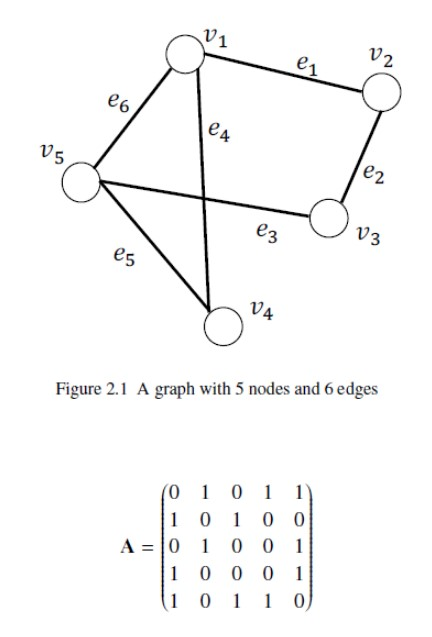
\includegraphics[width=0.5\textwidth]{2/MT/6.jpg}
		\caption{Propiedades u medidas de un grafo \\
			Fuente: \citep*{bk_grafo}. \citetitle{bk_grafo}. (p. 19)}
		\label{1:fig2}
	\end{center}
\end{figure}
%\medskip

Otro aspecto que conforma un grafo es su Matriz de Adyacencia, el cual se denota como $A \in \{0, 1\}$$NxN$. Cada $A_{ij}$ representa la relación que hay entre dos nodos. Cabe mencionar que, en un grafo no dirigido, su matriz de adyacencia es simétrica, es decir, $A_{ij} = A_{ji}$  \parencite{bk_grafo}.


\subsubsection{Propiedades de un grafo}
\subsubsection{Procesamiento de señales de Grafos}
\subsubsection{Transformación de Fourier en Grafos (GFT)}
\subsubsection{Tipo de Grafos}




\subsection{Métodos de Redes Neuronales Profundas basadas en Grafos}
\subsubsection{Graph Neural Networks}


\subsubsection{Robust Graph Neural Networks}
Al igual que las DNNs tradicionales, estas son vulnerables a ataques adversarios, generando perturbaciones en la manipulación de la estructura del grafo y la características de los nodos para engañar a los modelos de GNNs. Por esta limitación, Robusta Graph Neural Networks es una extensión de las GNNs que adoptan medidas críticas de seguridad, las cuáles pueden estar presentes en los sistemas financieros y la gestión de riesgo. La RGNNs comunmente utiliza un enfoque de limpieza del grafo perturbado, los cuáles han sido victimas de una violación de ciertas propiedades que presenta el grafo real 


\subsubsection{Scalable Graph Neural Networks}
Las GNNs tradicionales presentan problemas de escalabilidad que impide la adopción de grados a gran escala, debido a que utiliza un método de gradiente para minimizar la función de pérdida en cada etapa de representación de nodos, requiriendo una gran cantidad de recursos computacionales y operaciones de cálculos (Libro). Para abordar dichos problemas, se utilizan las técnicas y enfoques de las SGNNs para que las GNNs sean más eficientes a medida que el tamaño y la complejidad de los grafos van aumentando. Una de las principales técnicas de las SGNNs es el Graph Coarsening que utiliza la reducción de grafos para el entrenamiento escalable de estas (https://arxiv.org/abs/2106.05150).



\section{Marco Conceptual}
Para de


%\chapter{METODOLOGÍA DE LA INVESTIGACIÓN}
\section{Diseño de la investigación}
El diseño del presente trabajo de investigación es de tipo experimental puro, ya que se analizarán las variables, procesando los valores con técnicas de regresión para obtener un vector característico que sirva como entrada al modelo de Aprendizaje Profundo, específicamente un modelo de Redes Neuronales Profundas basadas en Grafos.
%Para finalizar se explicará el
%proceso de aplicación de las redes neuronales convolucionales.
\subsection{Tipo de investigación}
El tipo de investigación del presente trabajo es de alcance experimental, ya que el desarrollo de un algoritmo de Aprendizaje Profundo para la detección de rutas seguras en la ciudad de Los Ángeles busca una explicación a partir de patrones que predigan qué rutas son las más seguras basándose en los datos de geolocalización de incidentes delictivos; para ello, se establece una relación de causa efecto, donde a través de una función de riesgo determine qué rutas debe evitar para determinar la opción más segura.


\subsection{Enfoque de investigación}
El enfoque que presenta este trabajo es cuantitativo, ya que utiliza instrumentos de identificación y medición de riesgo en los datos de incidencias, cuyo resultado numérico servirá para entrenar al modelo de Aprendizaje Profundo para detectar qué rutas debe evitar.
\medskip

\section{Población y muestra}
\medskip
\begin{table}[h!]
	\centering
	\begin{tabular}{|m{4cm}|m{10cm}|}
		\hline
		\textbf{Categoría} & \textbf{Descripción} \\
		\hline
		\textbf{Población} & Registro de crímenes extraídos de la página oficial del Departamento de Policía de Los Ángeles, Estados Unidos, desde el año 2020 hasta el año 2024. \\
		\hline
		\textbf{Muestra} & Aproximadamente más de 680,000 registros de crímenes de la página oficial del Departamento de Policía de Los Ángeles. Para la selección de la muestra, se utilizó muestreo no probabilístico o dirigido, ya que se seleccionaron los registros que tienen como descripción aquellos crímenes perpetuados en las calles, tiendas o bancos; como por ejemplo asaltos a mano armada, violación, robo de vehículos, acoso sexual, vandalismo, entre otros. \\
		\hline
		\textbf{Unidad de análisis} & Latitud y Longitud donde ocurrió el crimen registrado. \\
		\hline
		\textbf{Variable y tipo de análisis} & Variable cuantitativa discreta, ya que el presente trabajo se centra en variables numéricas y la medición de riesgo de las rutas. \\
		\hline
	\end{tabular}
\end{table}
\medskip

\section{Operacionalización de Variables}
\medskip
\begin{table}[h!]
	\centering
	\small
	\begin{tabularx}{\textwidth}{|X|X|X|}
		\hline
		\multicolumn{3}{|c|}{\textbf{DEFINICIÓN DE VARIABLES}} \\
		\hline
		\textbf{VARIABLE Y DEFINICIÓN} & \textbf{INDICADOR} & \textbf{FÓRMULA} \\
		\hline
		RUTAS SEGURAS\newline Trayecto el cual evita las zonas con alto nivel de delincuencia para una persona. & Indicador de Riesgo & $R = \sum _{i=1}^{n}(W_{i}\times C_{i})$\newline Donde: 
		\begin{itemize}
			\item $n$ es el número de factores considerados.
			\item $W_{i}$ son los pesos asignados a cada factor.
			\item $C_{i}$ son los valores normalizados de cada factor.
		\end{itemize} \\
		\hline
		\multirow{3}{\hsize}{ALGORITMO DE APRENDIZAJE PROFUNDO\newline Tipo de algoritmo de la subcategoría del Aprendizaje Automático, el cual es el Aprendizaje Profundo, que utiliza Redes Neuronales Artificiales con múltiples capas para el procesamiento y análisis de datos complejos.} & Indicador de Eficiencia & $TTM = N_{ep} \times T_{ep}$ \newline Donde: 
		\begin{itemize}
			\item $N_{ep}$ es el número de épocas del modelo.
			\item $T_{ep}$ el tiempo promedio necesario para completar una época en el entrenamiento.
		\end{itemize}\\
		\cline{2-3}
		& Indicador de Precisión & $RMSE = \sqrt{\frac{1}{n}\sum _{i = 1}^{n}(y_{i}-\hat{y}_{i})^{2}}$ \newline Donde: 
		\begin{itemize}
			\item $n$ es el número total de observaciones o datos.
			\item $y_{i}$ es el valor observado en la posición $i$.
			\item $\hat{y}_{i}$ es el valor predicho en la posición $i$.
		\end{itemize}\\
		\cline{2-3}
		& Tasa de éxito del agente & $Success\: Rate = \frac{Number\,of \, Successful\,Routes}{Total\,Number\,of \, Routes}$ \\
		\hline
	\end{tabularx}
\end{table}
\medskip
\section{Técnicas de recolección de datos}
Para el presente trabajo se recolectó un conjunto de datos de registros públicos de crímenes en la ciudad de Los Ángeles, que se componen de variables tanto cuantitativas (longitud, latitud, fecha, área, número de documento, edad, entre otros), como cualitativas (descripción del crimen, dirección, sexo, entre otros). Para obtener este conjunto de datos se siguió un flujo de búsqueda, descarga y segmentación de los registros de crímenes en base al tipo de crimen realizado como se muestra en la figura. Cabe mencionar que en proceso de segmentación, el conjunto de datos contiene una columna llamada “Crm Cd Desc”, que son los tipos de crímenes registrados, por lo que se filtra aquellos crímenes que involucren agresión física o verbal, como también vandalismos en las zonas urbanas de una ciudad. Asimismo, se extraerá en formato XLSX solo las columnas necesarias para el entrenamiento del modelo, los cuáles son: Crm Cd Desc, Date Rptd, LAT, LON. “LAT” y “LON” representan la latitud y longitud donde ocurrió el crimen.
\medskip
\begin{figure}[h]
	\begin{center}
		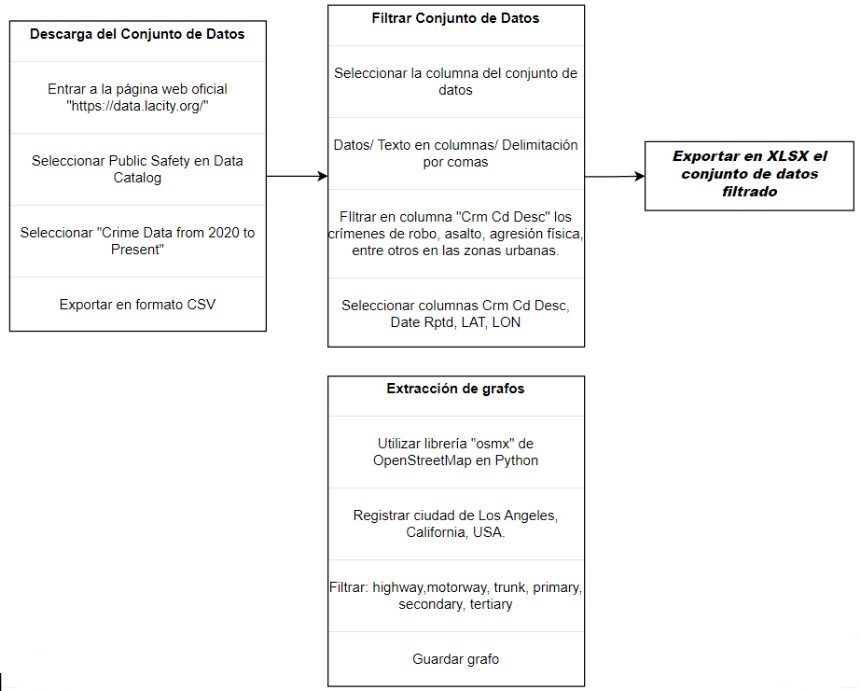
\includegraphics[width=0.7\textwidth]{3/figures/flujoreco.jpg}
		\caption[Elaboración propia: Flujo de recolección de datos]{Elaboración propia: Flujo de recolección de datos}
		\label{1:fig}
	\end{center}
\end{figure}
\medskip
Además de la extracción del conjunto de datos de registro de crímenes, es importante extraer la cartografía de la ciudad de Los Ángeles, como se muestra en la figura, haremos uso de la librería “osmnx” de OpenStreetMaps en Python para extraer los datos de una zona que buscas según lo que necesitas. Para el presente trabajo, se busca la región de la ciudad de Los Ángeles, el cual la librería nos brindará todas los nodos que son las calles, estaciones, avenidas, entre otros.

\section{Técnicas para el procesamiento y análisis de la información}
Para la metodología propuesta, se usó de base la metodología CRISP-DM(Cross-Industry Standard Process for Data Mining), que está orientado mayormente al campo de la minería de datos, es un proceso o un ciclo de vida del desarrollo de un modelo, y el cuál es altamente personalizable y flexible en cualquier tipo de situación o desarrollo \parencite{gl_crisp}. Este ciclo de vida del modelo consta de 6 fases, las cuales son:

%\begin{enumerate}
%	\item Like this,
%	\item and like this.
%\end{enumerate}
\begin{itemize}
	\item Entendimiento del modelo: La comprensión de los objetivos y requisitos definidos del proyecto para el usuario final, con el fin de convertir dicho conocimiento en una definición técnica del problema.
	\item Comprensión de los datos: Se realiza un análisis exploratorio en los datos para tener una visión general de lo que se puede conseguir de estas.
	\item Preparación de los datos: En esta fase se cubre todas las actividades requeridas para la construcción del conjunto de datos, junto con el preprocesamiento de los datos que serán empleados para la siguiente fase.
	\item Modelado de datos: Fase el cuál tiene que ver con la implementación de los modelos requeridos del proyecto que derivarán a los próximos resultados y conclusiones de este.
	\item Evaluación: Se mide los resultados y calidad del modelo, junto con su efectividad para el cumplimiento de los requisitos establecidos.
	\item La implementación del modelo en un entorno operativo, la planificación del mantenimiento y monitoreo de este para que siga cumpliendo con los objetivos del proyecto.
\end{itemize}
Estableciendo la base teórica en lo que consiste la metodología CRISP-DM, también se usó de ejemplo la metodología propuesta por \citeauthor{pr_saferoute} en su artículo \citetitle{pr_saferoute}, ya que estos trabajan también con conjuntos de datos de delitos y la obtención del mapa de las ciudades en OpenStreetMaps, además que implementa una función de recompensa basada en riesgos para entrenar su modelo de Aprendizaje por Refuerzo. Otro artículo de inspiración para el desarrollo de la metodología, es de \citeauthor{pr_esquivel} en su artículo \citetitle{pr_esquivel}, ya que proponen la aplicación de regresión LOESS para el preprocesamiento de los datos que serán utilizadas para el entrenamiento de su modelo LSTM basado en grafos. Por último, también tomará de guía el flujo de condición para la elección de rutas seguras propuesta por \citeauthor{pr_Soni} en su artículo \citetitle{pr_Soni}. La metodología del presente trabajo de investigación se puede visualizar de manera gráfica en la Figura \ref{1:mark}.\medskip

\begin{figure}[h]
	\begin{center}
		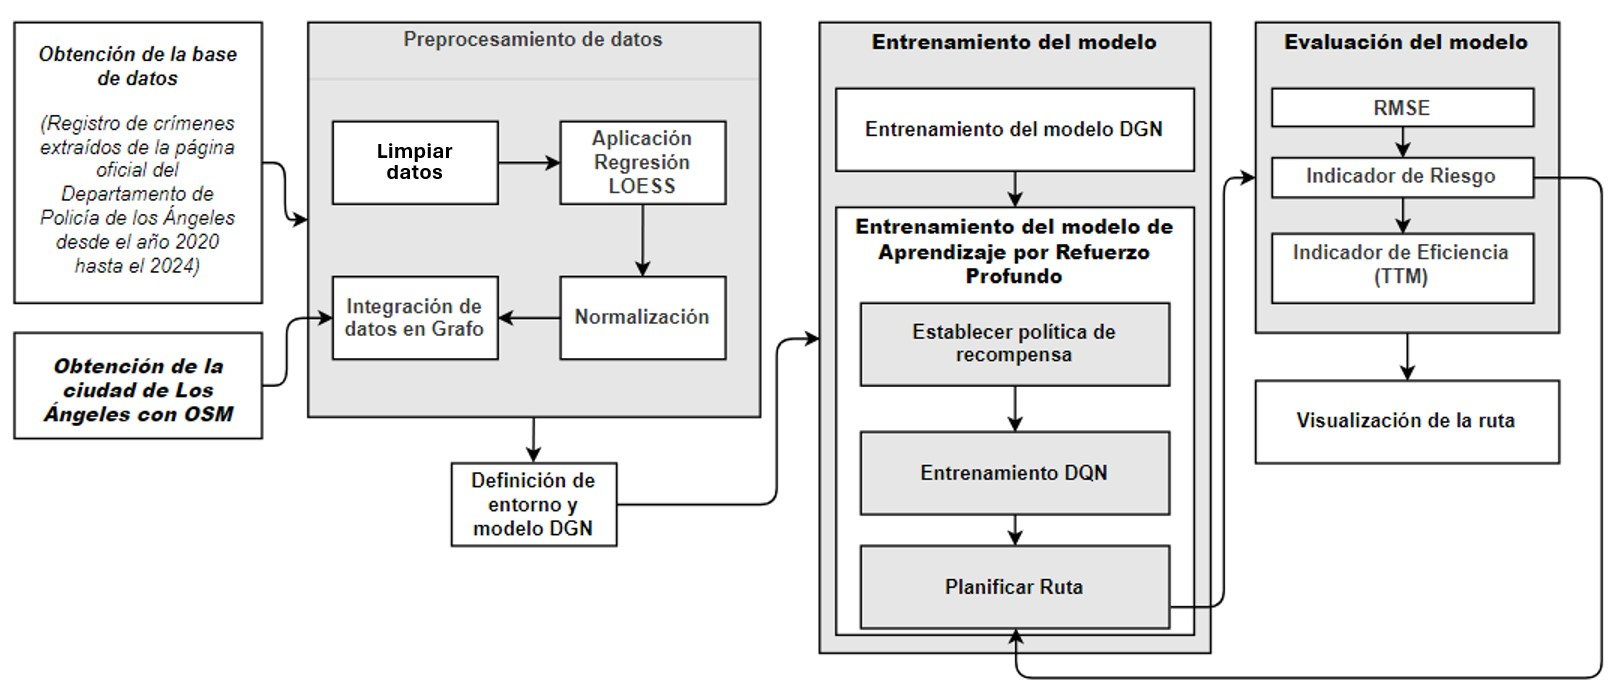
\includegraphics[width=0.7\textwidth]{3/figures/metopropuesta.jpg}
		\caption[Elaboración propia: Metodología propuesta]{Elaboración propia: metodología propuesta}
		\label{1:mark}
	\end{center}
\end{figure}
\medskip
Como ya se mencionó, esta metodología viene de la derivación de la metodología tradicional CRISP-DM junto con las metodologías propuestas en los antecedentes. Se puede encontrar una relación entre la comprensión del negocio con el objetivo del presente artículo el cuál es la minimización del riesgo en la detección de rutas seguras. Asimismo, en la fase de la comprensión de los datos, se encuentra la recolección de los registros de crímenes en la ciudad de Los Ángeles y la obtención de la ciudad de Los Ángeles en OpenStreetMap. La fase de preparación de los datos es más que la fase del preprocesamiento de los datos con sus respectivos pasos propuestos por la metodología. Mientras que el Modelado es la creación y entrenamiento del modelo de Deep Graph Network (DGN) para la representación del grafo de la ciudad y del entrenamiento del modelo de Aprendizaje por Refuerzo Profundo para establecimiento de las políticas de recompensa y la planificación y detección de rutas seguras. Por último, las fases de evaluación y despliegues son las métricas propuestas en la metodología que determinará qué ruta segura debe elegir el usuario según el índice de riesgo que presente.
\subsection{Metodología de la implementación de la solución}
\subsubsection{Adquisición}
En esta fase se describe la obtención del conjunto de datos, como ya se mencionó anteriormente en el punto de las técnicas de recolección, se necesita registros de crímenes realizados en una zona urbana, para esto, se decidió trabajar con el conjunto de datos abiertos de registros de crimen en la ciudad de Los Ángeles desde el 2020 hasta el 2024. Dicho conjunto de datos tiene más de novecientos veinticinco mil registros aproximadamente y cuenta con 28 columnas las cuáles se detallan a continuación:


\begin{longtable}{|p{2.5cm}|p{6cm}|p{5cm}|}
	\hline
	\textbf{Nombre de Columna} & \textbf{Descripción} & \textbf{Tipo de dato} \\
	\hline
	\endfirsthead
	
	\multicolumn{3}{c}{{\tablename\ \thetable{} -- Continuación de la página anterior}} \\
	\hline
	\textbf{Nombre de Columna} & \textbf{Descripción} & \textbf{Tipo de dato} \\
	\hline
	\endhead
	
	\hline
	\multicolumn{3}{r}{{Continúa en la siguiente página}} \\
	\endfoot
	
	\hline
	\caption{Descripción de las columnas del conjunto de datos de LAPD \\
		Fuente: \citep*{gl_LAPD}. \citetitle{gl_LAPD}.} \label{tab:lapd-data-description} \\
	\endlastfoot
	
	DR\_NO & Número de División de Registros: Número de archivo oficial compuesto por un año de 2 dígitos, un ID de área y 5 dígitos & Texto \\
	\hline
	Date Rptd & MM/DD/YYYY Floating Timestamp & Texto \\
	\hline
	DATE OCC & MM/DD/YYYY Floating Timestamp & Texto \\
	\hline
	TIME OCC & En horario militar de 24 horas & Texto \\
	\hline
	AREA & El LAPD tiene 21 comisarías comunitarias denominadas áreas geográficas dentro del departamento. & Texto \\
	\hline
	AREA NAME & Las 21 áreas geográficas o divisiones de patrulla también reciben una designación de nombre que hace referencia a un punto de referencia o a la comunidad circundante. & Texto \\
	\hline
	Rpt Dist No & Un código de cuatro dígitos que representa una subárea dentro de un Área Geográfica. & Texto \\
	\hline
	Part 1-2 & Sin descripción & Número \\
	\hline
	Crm Cd & Indica el delito cometido. (Igual que el Código Penal 1) & Texto \\
	\hline
	Crm Cd Desc & Define el Código Penal previsto. & Texto \\
	\hline
	Mocodes & Modus Operandi: actividades asociadas con el sospechoso en la comisión del delito. & Texto \\
	\hline
	Vict Age & Numérico de dos caracteres & Texto \\
	\hline
	Vict Sex & F - Mujer M - Hombre X - Desconocido & Texto \\
	\hline
	Vict Descent & Código de ascendencia: A - Otro asiático ... Z - Indio asiático & Texto \\
	\hline
	Premis Cd & El tipo de estructura, vehículo o lugar donde ocurrió el delito. & Número \\
	\hline
	Premis Desc & Define el Código de Premisa proporcionado. & Texto \\
	\hline
	Weapon Used Cd & El tipo de arma utilizada en el delito. & Texto \\
	\hline
	Weapon Desc & Define el código de arma utilizada proporcionado. & Texto \\
	\hline
	Status & Estado del caso. (IC es el valor predeterminado) & Texto \\
	\hline
	Status Desc & Define el código de estado proporcionado. & Texto \\
	\hline
	Crm Cd 1 & Indica el delito cometido. El Código Penal 1 es el principal y el más grave. & Texto \\
	\hline
	Crm Cd 2 & Puede contener un código para un delito adicional, menos grave que el Código Penal 1. & Texto \\
	\hline
	Crm Cd 3 & Puede contener un código para un delito adicional, menos grave que el Código Penal 1. & Texto \\
	\hline
	Crm Cd 4 & Puede contener un código para un delito adicional, menos grave que el Código Penal 1. & Texto \\
	\hline
	LOCATION & Dirección del incidente del crimen redondeada a la centena de cuadra más cercana para mantener el anonimato. & Texto \\
	\hline
	Cross Street & Cruce de Calle de Dirección Redondeada & Texto \\
	\hline
	LAT & Latitud & Número \\
	\hline
	LON & Longitud & Número \\
	\hline
\end{longtable}

Dicho conjunto de datos se seleccionarán las columnas importantes que servirán para el entrenamiento del modelo propuesto, los cuáles son las columnas Crm Cd Desc, Date Rptd, LAT y LON. Con respecto al tipo de crimen, este conjunto de datos contiene múltiples registros que van desde vandalismo callejero a fraude financiero, por lo que se decidió filtrar manualmente en la columna Crm Cd Desc lo siguiente: VEHICLE - STOLEN, BURGLARY FROM VEHICLE, BIKE - STOLEN, SHOPLIFTING-GRAND THEFT (\$950.01 \& OVER), BATTERY - SIMPLE ASSAULT, CRM AGNST CHLD (13 OR UNDER) (14-15 \& SUSP 10 YRS OLDER), ASSAULT WITH DEADLY WEAPON, AGGRAVATED ASSAULT,	CRIMINAL THREATS - NO WEAPON DISPLAYED, THEFT FROM MOTOR VEHICLE - PETTY (\$950 \& UNDER)	BURGLARY, THEFT PLAIN - PETTY (\$950 \& UNDER), THEFT FROM MOTOR VEHICLE - GRAND (\$950.01 AND OVER), ROBBERY, BUNCO, GRAND THEFT, BATTERY WITH SEXUAL CONTACT, SHOPLIFTING - PETTY THEFT (\$950 \& UNDER), VANDALISM - FELONY (\$400 \& OVER, ALL CHURCH VANDALISMS), RAPE, FORCIBLE, VANDALISM - MISDEAMEANOR (\$399 OR UNDER), OTHER ASSAULT, PICKPOCKET, DISTURBING THE PEACE, BUNCO, ATTEMPT, PEEPING TOM, ATTEMPTED ROBBERY, CHILD STEALING, INDECENT EXPOSURE, STALKING, BURGLARY, ATTEMPTED, RAPE, ATTEMPTED, DISCHARGE FIREARMS/SHOTS FIRED, VEHICLE - ATTEMPT STOLEN, BURGLARY FROM VEHICLE, ATTEMPTED	THEFT, PERSON, VEHICLE, STOLEN - OTHER (MOTORIZED SCOOTERS, BIKES, ETC), THEFT FROM PERSON - ATTEMPT, BOMB SCARE, ASSAULT WITH DEADLY WEAPON ON POLICE OFFICER, SHOTS FIRED AT INHABITED DWELLING	KIDNAPPING - GRAND ATTEMPT, SHOTS FIRED AT MOVING VEHICLE, TRAIN OR AIRCRAFT, THROWING OBJECT AT MOVING VEHICLE	KIDNAPPING, CRIMINAL HOMICIDE, PURSE SNATCHING, THEFT FROM MOTOR VEHICLE - ATTEMPT, SHOPLIFTING - ATTEMPT, PROWLER, MANSLAUGHTER, NEGLIGENT, PURSE SNATCHING - ATTEMPT, BIKE - ATTEMPTED STOLEN, PICKPOCKET, ATTEMPT.

Todos los tipos de crímenes mencionados están relacionados con robos, asaltos, vandalismo, agresión física o sexual en las zonas públicas, asalto a pequeñas tiendas, acoso, intento de robo, entre otros. La principal razón por la que se debe filtrar este tipo de crímenes es para que el modelo pueda predecir las rutas seguras en base a crímenes perpetrados en las calles. Esto da más de seiscientos mil registros.

\textbf{Entregable:} Conjunto de datos con columnas requeridas para el entrenamiento del modelo filtrado por crímenes ocasionados en las calles de la ciudad.

Además de la adquisición del conjunto de datos, se debe obtener el mapa de la zona de la ciudad de Los Ángeles, con el fin de tener las calles, avenidas, estaciones y vías que servirá al modelo para la creación del grafo. Para esto se hará uso de la librería de OpenStreetMap llamada “OSMX” y qué en base a una consulta realizada en Python filtrado con los parámetros "highway", "motorway”, “trunk”, “primary”, “secondary”, “tertiary" , se obtendrá los nodos y vértices de la ciudad.

\textbf{Entregable:} Grafo de las calles de la ciudad de Los Ángeles obtenidos de la librería OSMX.
\medskip

\begin{figure}[h]
	\begin{center}
		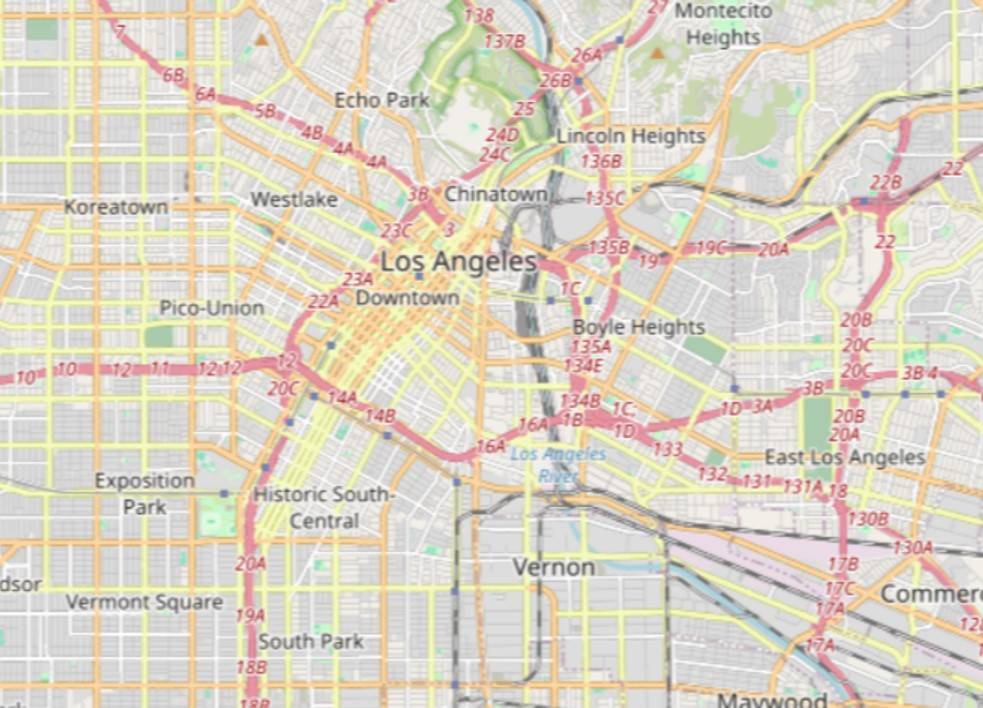
\includegraphics[width=0.65\textwidth]{3/figures/grafoa.jpg}
		\caption[Zona de la ciudad de Los Ángeles en OpenStreetMap]{Zona de la ciudad de Los Ángeles en OpenStreetMap}
		\label{1:fig}
	\end{center}
\end{figure}
\medskip

\subsubsection{Preprocesamiento de datos}

En esta fase se realizará 4 pasos para que la carga de la información esté lista y limpia para hacer su uso en la etapa de entrenamiento del modelo, por lo que se detallará a continuación los siguientes pasos.

\begin{itemize}
	\item[a.] Limpieza de dato \\

Este primer paso ayudará en primera instancia a eliminar los datos vacíos que se encuentran en la base de datos de registro de crímenes. Esto puede causar problemas a la hora de entrenar el modelo y reducir la precisión de este, por lo que es esencial mantener la integridad del conjunto de datos, para esto, Python cuenta con múltiples librerías o lista de comandos que le permite eliminar los datos faltante según los parámetros que se le imponga, una de las más conocidas es “.dropna()”.

El segundo paso el cambio de tipo de variable, ya que el conjunto de datos está compuesto mayoritariamente por variables de tipo texto que no deberían ser consideradas de esa manera, hacer un correcto cambio en el tipo de variables permitirá hacer un análisis de series de tiempo más eficiente y preciso o aplicarla correctamente en los pasos posteriores como la aplicación de regresión LOESS.  Python también ofrece múltiples listas de comandos que permiten cambiar el tipo de variable según las necesidades requeridas del proyecto.

\textbf{Entregable:} Conjunto de datos completo con la correcta clasificación de sus variables.
	\item[b.] Aplicación Regresión LOESS \\
	
La Regresión LOESS	es un método que combina la regresión lineal con la regresión no lineal, ajustando modelos sencillos sobre subconjuntos locales de datos para la creación de una función que describa la variación de los datos. En cada punto del conjunto de datos se ajusta una regresión polinómica dando más peso a los puntos cercanos y menos peso a los más lejanos, esto puede ayudar para la determinar la relación entre entre las variables y sobre todo, el manejo de datos ruidosos, es decir, si presenta una gran variabilidad en los datos, por lo que puede resaltar las tendencias para entender mejor las áreas donde hay más crímenes, proporcionando una visión más clara de los patrones de los datos y mejorando la identificación de zonas de alto riesgo \parencite{gl_maxima}.

Para esto, se selecciona primero cada punto de interés Xi, para la asignación de pesos se utiliza la siguiente fórmula:

\begin{equation} 
	w_{i}(x)=(1-\begin{vmatrix}
		\frac{x-x_{i}}{d_{max}}
	\end{vmatrix}^{3})^{3}
\end{equation}

Donde $d_{max}$ es la distancia máxima dentro del vecindario.
Adicionalmente a esto, se realiza el ajuste del Polinomio local en término de matrices, el cual se hace minimizando la suma ponderada de los errores cuadrado:

\begin{equation} 
	\sum_{i}w_{i}(x)(y_{i}-(\beta _{0}+\beta _{1}(x_{i}-x)))^{2}
\end{equation}

Donde $y_{i}$ son los valores de respuesta.

\textbf{Entregable:} Conjunto de datos suavizados de los crímenes con baja variabilidad de estos.

	\item[c.] Normalización \\

Dado a que se trabaja con la latitud y longitud, es importante el proceso de la normalización para que tengan una escala similar, esto ayuda a mejorar la eficiencia y precisión del modelo. Se hará uso de la normalización Min-Max, ya que asegura que todos los atributos están el el rango de 0 a 1, asimismo ayuda a preservar las relaciones entre los valores originales y es compatible con muchos algoritmos\parencite{gl_med}. 
	\begin{equation} 
		{x}'=\frac{x-x_{min}}{x_{max}-x_{min}}
	\end{equation}

Donde:

$x$ es el valor original.

$x_{min}$ es el valor mínimo de la característica.

$x_{max}$ es el valor máximo de la característica.

${x}'$ es el valor normalizado.

\textbf{Entregable:} Conjunto de datos normalizados en un mismo rango.
	
	\item[d.] Normalización \\
	
Este paso es necesario para el análisis y toma de decisiones del modelo, por lo que se debe contar con la estructura geográfica de la ciudad representada en grafo de OpenStreetMap, junto con el conjunto de datos ya normalizados. Para la evaluación del riesgo de una ruta, se debe asociar cada registro de crimen con el vértice más cercano (intersección) o con la arista (calle) dónde ocurrió en la ciudad, para esto se utiliza la distancia euclidiana, el cual se representa de la siguiente manera:

\begin{equation} 
	d=\sqrt{(x_{2}-x_{1})^{2}+(y_{2}-y_{1})^{2}}
\end{equation}

Dónde $(x_{1},y_{1})$ son las coordenadas del crimen y $(x_{2},y_{2})$ son las coordenadas del vértice del grafo.

\textbf{Entregable:} Conjunto de datos integrado en el grafo de la ciudad para su uso en la fase de entrenamiento.

\end{itemize}

\subsubsection{Definición de entorno y modelo DGN}

La definición de un entorno para el entrenamiento del modelo es fundamental para proporcionar una plataforma robusta y flexible para encontrar rutas seguras en el grafo de la ciudad, para esto se hará uso del entorno Gym, que es un paquete proporcionado por Python y que da la facilidad de establecer reglas y la capacidad de interactuar con el entorno del grafo de la ciudad para la toma de decisiones y recibir recompensas basadas en el riesgo \parencite{gl_gym}. Asimismo, Gym puede facilitar la implementación de algoritmos DGN y diferentes algoritmos DRL, además de ser compatibles con diversas bibliotecas de Aprendizaje Profundo como TensorFLow, Pytorch, entre otros que facilita la integración de los algoritmos de DRL como DQN.
Para la elección de un modelo DGN, se optó por utilizar el modelo Graph Convolutional Network (GCN), por su capacidad de modelar relaciones complejas entre los nodos y aristas en grafos para saber cómo están distribuidos los crímenes a lo largo de las calles y vecindarios. Asimismo, GCN tiene la capacidad de procesar eficientemente datos espaciales en el grafo que le permite integrar los datos de los registros de crímenes ya que se manejan según coordenadas. Debido a que la ciudad de Los Ángeles está compuesta por muchas calles y avenidas que se interceptan entre sí, esto hace que sea un grafo grande y complejo, el cual un modelo GCN es flexible y adaptable a ese sin necesidad de establecer características específicas \parencite{gl_git}.
\medskip

\begin{figure}[h]
	\begin{center}
		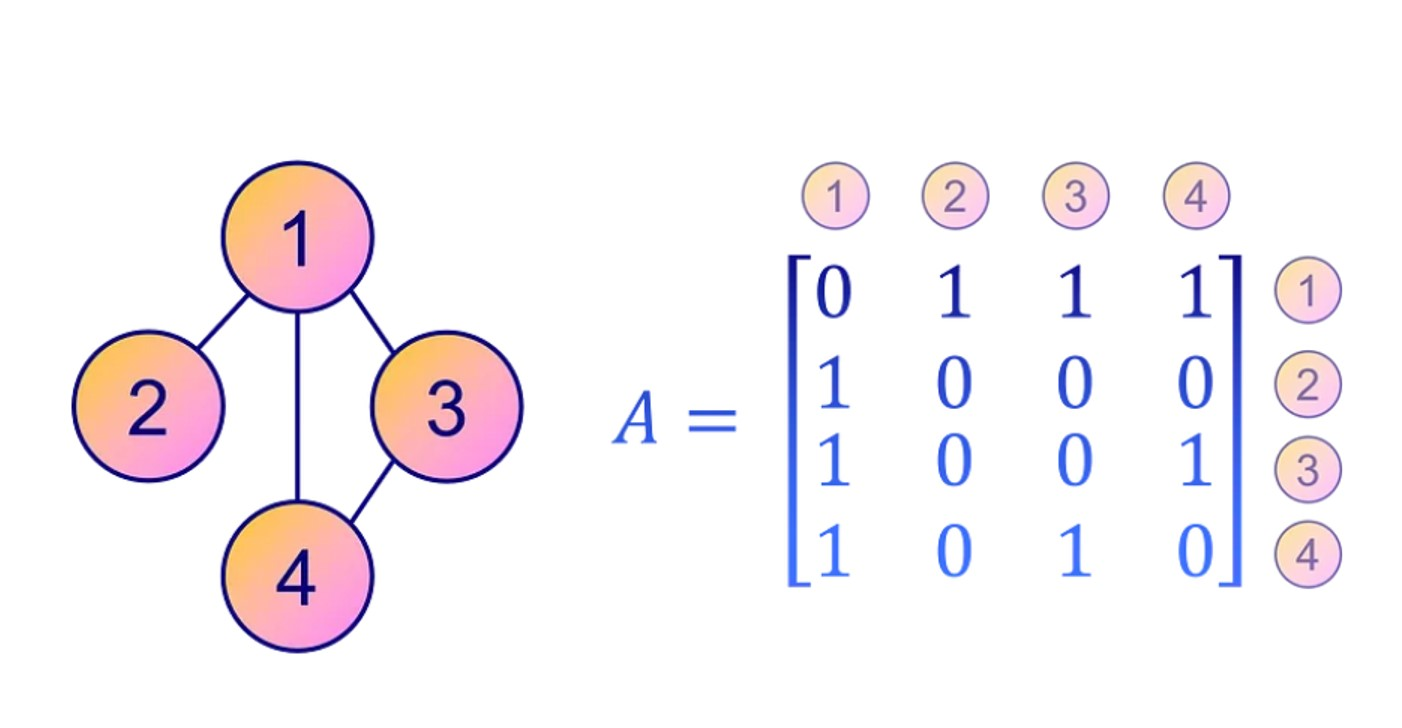
\includegraphics[width=0.65\textwidth]{3/figures/grafosim.jpg}
		\caption[Estructura simple de un grafo]{Estructura simple de un grafo\\
			Fuente: \citep*{gl_gnnmed}. \citetitle{gl_gnnmed}.}
		\label{1:fig}
	\end{center}
\end{figure}
\medskip
\textbf{Entregable:} Entorno de trabajo en Gym utilizando el modelo GCN para la fase del entrenamiento.

\subsubsection{Entrenamiento del Modelo}

Para el entrenamiento del modelo DGN, este será realizado en el entorno de TensorFlow, el cual permite la construcción de modelos de Aprendizaje Profundo complejos y personalizados, definiendo capas personalizadas, funciones de activación y de pérdida. Otra de las razones es porque está optimizado para realizar cálculos en grandes volúmenes de datos y que está respaldado por Google y una gran comunidad de desarrolladores, brindándonos abundante contenido y documentación para la implementación efectiva del GCN
\begin{itemize}
	\item[a.] Entrenamiento del modelo DGN \\
	
Para el entrenamiento del modelo DGN, este será realizado en el entorno de TensorFlow, el cual permite la construcción de modelos de Aprendizaje Profundo complejos y personalizados, definiendo capas personalizadas, funciones de activación y de pérdida. Otra de las razones es porque está optimizado para realizar cálculos en grandes volúmenes de datos y que está respaldado por Google y una gran comunidad de desarrolladores, brindándonos abundante contenido y documentación para la implementación efectiva del GCN.
\medskip

\begin{figure}[h]
	\begin{center}
		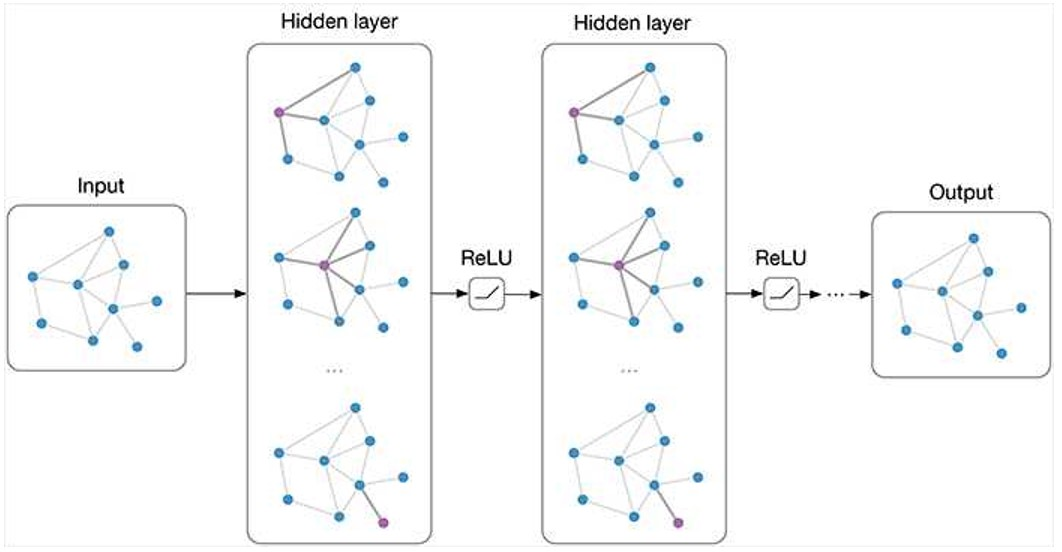
\includegraphics[width=0.65\textwidth]{3/figures/estru.jpg}
		\caption[Estructura de GCN]{Estructura de GCN\\
			Fuente: \citep*{gl_aisummer}. \citetitle{gl_aisummer}.}
		\label{1:fig}
	\end{center}
\end{figure}
\medskip

En cuanto a las funciones de activación, se utilizará la función de activación ReLU (Rectified Linear Unit), ya que el modelo GCN requiere de funciones de activación no lineales para aprender y modelar las relaciones complejas entre los datos y mejora el rendimiento del modelo teniendo una mejor capacidad de identificar zonas de alto riesgo de crimen. Esta función de activación es representada matemáticamente como:

\begin{equation} 
	ReLU=max(0,x)
\end{equation}

Donde $x$ es un valor de entrada, y que la función devuelve 0 si en caso $x$ es negativo y si es positivo devuelve $x$.

Está función de activación ReLU será empleada en cada capa oculta del modelo.

En cuanto a la función de activación de la capa de salida, se utilizará la función Sigmoid, el cuál comprime los valores de entrada a un rango entre 0 y 1, útil para predecir la probabilidad de riesgo de crímen para cada nodo del grafo y que de esta manera el agente pueda determinar qué ruta tomar en modelo DRL. La función de activación es representada matemáticamente de la siguiente manera:

\begin{equation} 
	Sigmoid(x)=\frac{1}{1+e^{-x}}
\end{equation}

Se emplea la fórmula de propagación el cual permite actualizar las características de cada nodo en función de las características de sus vecinos, con el fin de capturar relaciones estructurales en el grafo, este aprenderá los pesos con el fin de minimizar la función de pérdida, ajustando para mejorar la predicción del riesgo. Esta fórmula es representada de la siguiente manera:

\begin{equation} 
	h_{v}^{l+1}=\sigma (\sum_{u \in  N(v)}\frac{1}{c_{uv}}h_{v}^{l}W^{l})
\end{equation}

Donde:

$h_{v}^{l}$ es la representación del nodo $v$ en la capa $l$.

$N(v)$ son los nodos vecinos de $v$.

$c_{uv}$ es el factor de la normalización de la arista entre $u$ y $v$.

$W^{l}$ es la matriz de pesos en la capa $l$.

$\sigma$ es la función de activación.

Por último se emplea un optimizador para el entrenamiento del modelo en TensorFlor, siendo el más conocido el Optimizador Adam (Adaptive Moment Estimation), que funciona en diversos problemas, ajustando automáticamente la tasa de aprendizaje en función se su estimación del momento \parencite{gl_interactive}.

\textbf{Entregable:} Representaciones de las características de riesgo de crimen en un grafo para el entrenamiento del modelo DRL y la probabilidad de riesgo de cada nodo.

\item[b.] Entrenamiento del modelo de Aprendizaje por Refuerzo Profundo \\
\begin{itemize}
	\item Establecer política de recompensa \\

Para el establecimiento de una política de recompensa, la cuál le servirá al agente determinar qué ruta será la más segura, se hará uso de las probabilidades de riesgo de cada nodo obtenidas en el entrenamiento del modelo DGN, además de establecer un umbral, que es de 0.6 y que representa el valor máximo que puede tomar el agente para elegir qué ruta tomar. Para esto, se propone la siguiente fórmula:

\begin{equation} 
	Recompensa = \left\{\begin{matrix}
		R_{safe}\; \; \; si\; Indice \;de\;Riesgo\;\leq \theta \\ 
		R_{risk}\; \; \; si\; Indice \;de\;Riesgo\;>  \theta 
	\end{matrix}\right.
\end{equation}

En cada nodo que el agente visite, este determinará mediante la función de recompensa si debe tomar dicho nodo, si en caso el índice de riesgo es menor al umbral, lo selecciona, caso contrario, lo evita.

\textbf{Entregable:} Función de recompensa para el entrenamiento del modelo DQN.

	\item Entrenamiento DQN \\

Para que el modelo aprenda a elegir la ruta más segura basándose en la política de recompensa ya establecida anteriormente, se decide entrenar un agente en un modelo DQN, ya que tiene la capacidad de manejar problemas de toma de decisiones mediante la interacción en entornos complejos y de alta dimensionalidad como lo es el grafo de la ciudad de Los Ángeles. Para el correcto entrenamiento del modelo DQN, se debe considerar los siguientes parámetros:
\begin{itemize}
	\item \textbf{Replay Buffer Size:} Este parámetro tiene como propósito el de almacenar las experiencias del agente, es decir, es una memoria que incluye el estado, la acción tomada, la recompensa recibida y el siguiente estado resultando, haciendo que el entrenamiento sea más estable y eficiente \parencite{gl_ray}. El tamaño que se define comúnmente es de 100,000 experiencias. Sin embargo, el establecimiento del tamaño de experiencia depende de la memoria y tiempo de muestreo durante el entrenamiento.
	\item \textbf{Minibatch Size:} Número de experiencias muestreadas del parámetro anterior de cada red neuronal y ayuda a estabilizar el aprendizaje con un correcto uso de los recursos computacionales. Los valores típicos son 32 o 64.
	\item \textbf{Learning rate:}  Es la tasa de aprendizaje del modelo y el encargado de ajustar o controlar el tamaño de los pesos de la red neuronal. El valor comúnmente utilizado es 0.001. Se debe evitar utilizar una tasa de aprendizaje mayor ya que puede volver inestable el modelo, asimismo, si la tasa es muy baja puede aumentar el tiempo de aprendizaje del modelo DRL \parencite{gl_findin}.
	\medskip
\begin{figure}[h]
	\begin{center}
		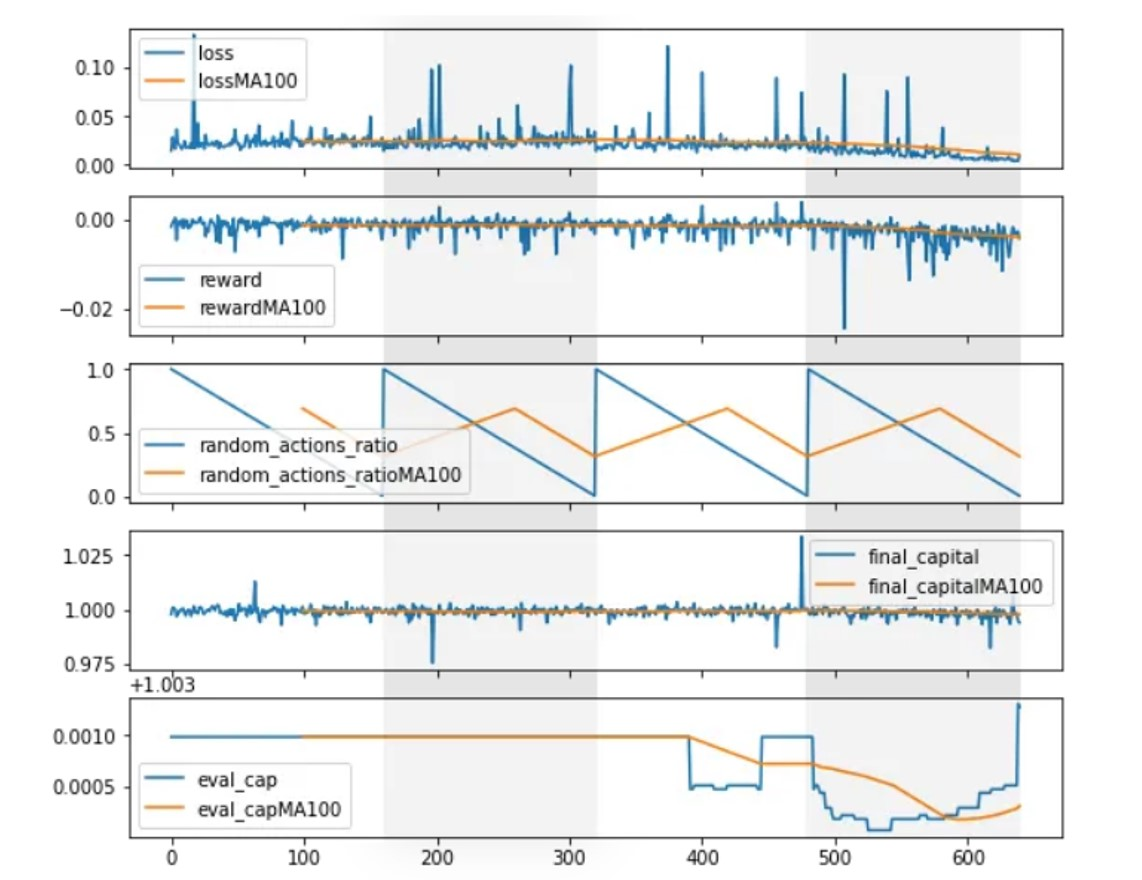
\includegraphics[width=0.65\textwidth]{3/figures/learning.jpg}
		\caption[Experimentación de tasa de aprendizajes]{Experimentación de tasa de aprendizajes\\
			Fuente: \citep*{gl_findin}. \citetitle{gl_findin}.}
		\label{1:fig}
	\end{center}
\end{figure}
\medskip
	
	\item \textbf{Discount Factor:} Determina la importancia de las recompensas, controlando la valoración que le asigna el agente a la recompensa frente a las recompensas futuras. El valor de recompensa varía de 0 a 1, siendo los valores típicos entre 0.9 y 0.99; este valor determina que tan importante es para el agente las recompensas futuras, por lo que sí es bajo, valorará más las recompensas inmediatas. Esto puede ayudar al modelo de detección de rutas seguras para saber si vale la pena seguir al siguiente nodo.
	\item \textbf{Exploration Rate:} Es un parámetro que controla la probabilidad de que el agente tome una acción, esto facilita el equilibrio entre la política aprendida y la exploración de nuevas acciones. Este paso es importante para el modelo, porque le permitirá explorar más las diversas calles de la ciudad, que serían los nodos, para que el agente descubra nuevas estrategias. Usualmente se inicia con un valor alto de 1 en exploración y mediante se va entrenando el modelo va disminuyendo gradualmente.
	
	\item \textbf{Target Network Update Frequency:} Es la frecuencia con la que se actualiza la red con el fin de estabilizar el entrenamiento con número de pasos establecidos. Se debe seleccionar la cantidad de pasos según lo requiera el modelo, ya que una frecuencia de actualización más alta puede hacer que la red se desactualice o si en caso es muy baja, se desestabilice el entrenamiento debido a los cambios realizados por la red. Los valores típicos suelen ser de 10000 pasos. 
		\medskip
	\begin{figure}[h]
		\begin{center}
			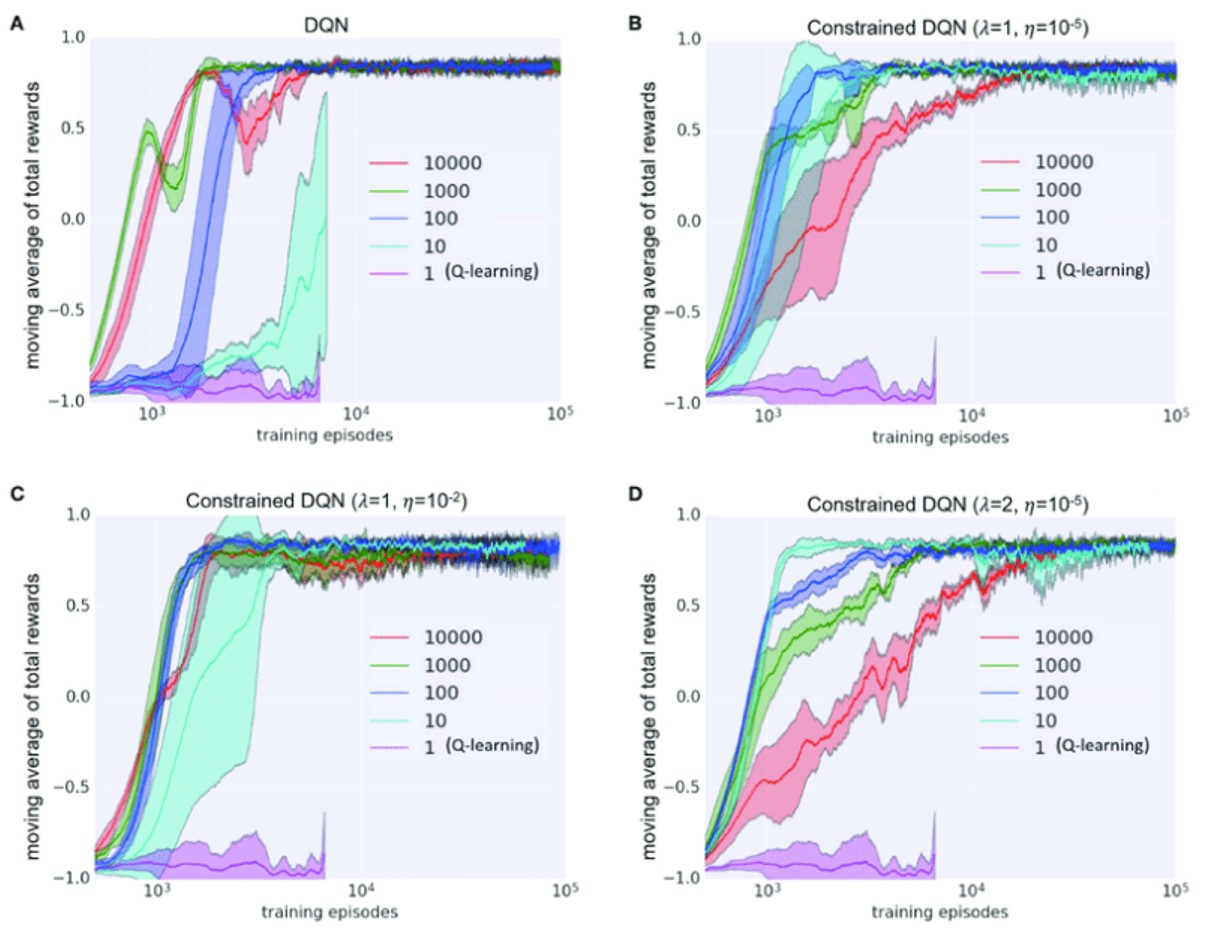
\includegraphics[width=0.7\textwidth]{3/figures/batch.jpg}
			\caption[Efectos de la frecuencia de actualización de la red objetivo en la tarea del laberinto MNIST]{Efectos de la frecuencia de actualización de la red objetivo en la tarea del laberinto MNIST\\
				Fuente: \citep*{gl_constr}. \citetitle{gl_constr}.}
			\label{1:fig}
		\end{center}
	\end{figure}
	\medskip
\end{itemize}
\textbf{Entregable:} Modelo DQN entrenado con una política optimizada de mapeo de estado del entorno a la acción que maximiza la recompensa esperada.

\end{itemize}
\item[c.] Planificar Ruta \\
Tomando en cuenta el entrenamiento del modelo DQN y la política optimizada, el agente utiliza dicha política desde el punto de origen para decidir el siguiente nodo en la ruta. Para esto, se utiliza una propagación hacia delante, donde cada paso que realiza el agente consulta a la política para saber si la acción minimiza el riesgo de crimen, asegurando que siempre se elija la mejor opción. Luego este proceso se realiza iterativamente hasta que el agente alcance el destino, construyendo una ruta completa y coherente. Además, se registra los índices de riesgo de cada nodo o arista seleccionada por el agente y se representa matemáticamente de la siguiente manera:
\begin{equation} 
	R_{total}=\sum_{i=1}^{N}r_{i}
\end{equation}
Donde $r_{i}$ es la probabilidad de riesgo de cada nodo o arista $i$, lo que proporciona una medida cuantitativa del riesgo para evaluar la efectividad del modelo.

\textbf{Entregable:} Subgrafo de la ruta resultante y el índice total de riesgo.

\end{itemize}

\subsection{Metodología para la medición de resultados}
\subsubsection{Evaluación del Modelo}
\begin{itemize}
	\item Root Mean Squared Error (RMSE)
	
	Se utiliza el RMSE para medir la precisión del modelo DGN propuesto en cuanto a las probabilidades de riesgo, cuantificando la desviación de las probabilidades de riesgo de cada nodo. Para esto, se utiliza la fórmula tradicional que es la siguiente:
	
\begin{equation} 
	RMSE = \sqrt{\frac{1}{N}\sum_{i=1}^{N}(y_{i}-\hat{y}_{i})^{2}}
\end{equation}
	
Donde:

$N$ es el total de nodos del grafo.

$y_{i}$ es la probabilidad de riesgo objetivo para nodo $i$.
	
$\hat{y}_{i}$ es la probabilidad de riesgo predicha por el modelo DGN para nodo $i$.
	
	Si el valor es bajo, quiere decir que las estimaciones de riesgo son precisas y asegura que el modelo propuesto es efectivo para la identificación de zonas de alto riesgo para que el agente pueda evitar dichas zonas en el proceso de entrenamiento DQN.
	
\textbf{Entregable:} Índice de efectividad del modelo DGN.
	\item Indicador de Riesgo \\
	Se utiliza la función de riesgo total establecido para la planificación de la ruta, y se evalúa el riesgo a cada ruta propuesta. Asimismo se establece un umbral que servirá de comparación con el riesgo total de una ruta, el cual determinará si la ruta se acepta o no. A continuación, se presenta el flujo condicional para la aceptación de la ruta:
	
	\begin{figure}[h]
		\begin{center}
			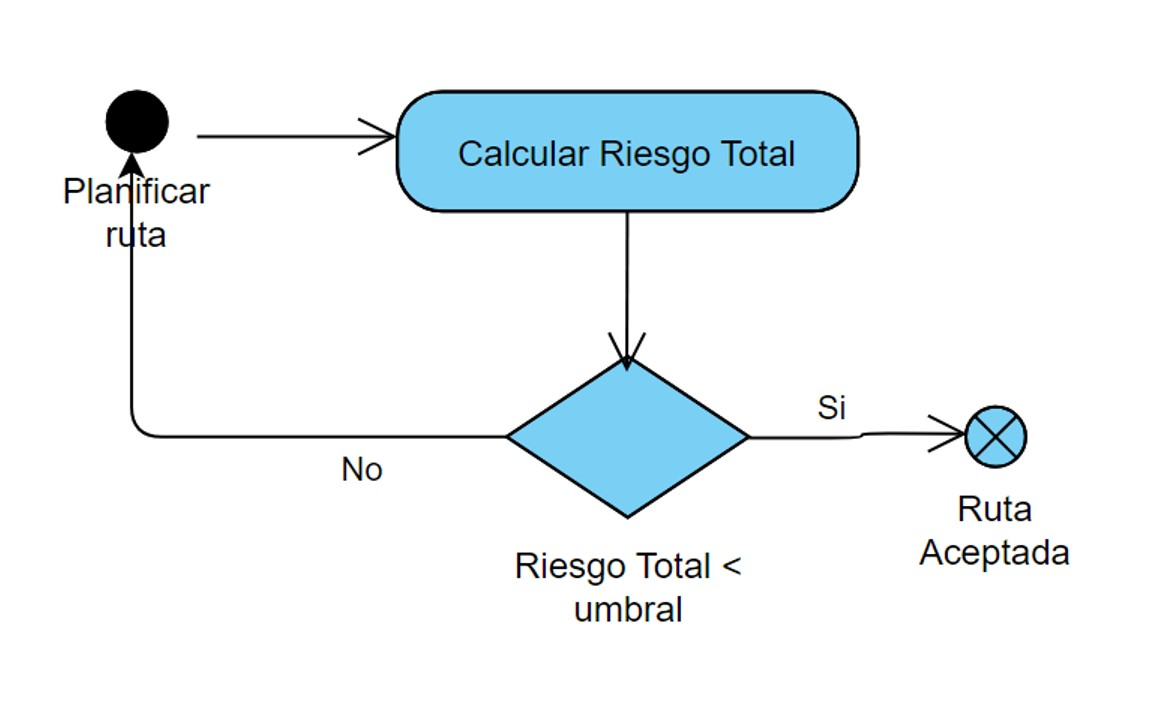
\includegraphics[width=0.65\textwidth]{3/figures/flujoCONDI.jpg}
			\caption[Elaboración propia: Flujo de condición de elección de ruta]{Elaboración propia: Flujo de condición de elección de ruta}
			\label{1:fig}
		\end{center}
	\end{figure}
	
\textbf{Entregable:} Ruta Segura con el menor índice de riesgo aceptada.
	\item Indicador de Eficiencia (TTM) \\
El indicador de Eficiencia (TTM) evalúa el rendimiento del modelo DRL, con el fin de proporcionar una medida cuantitativa para el tiempo de procesamiento del modelo y que se determina de la siguiente manera:
\begin{equation} 
	TTM = N_{ep} \times T_{ep}
\end{equation}

Donde: 

$N_{ep}$ es el número de épocas del modelo.

$T_{ep}$ el tiempo promedio necesario para completar una época en el entrenamiento.

Asimismo, se evalúa otro indicador de Eficiencia (TTM) que es para determinar el tiempo promedio de la ruta seleccionada, y puede ser representada de la siguiente manera:
\begin{equation} 
	TTM = \frac{Distancia \:de \:la\: ruta}{Velocidad \: Promedio}
\end{equation}
\textbf{Entregable:} Indicador de eficiencia del modelo DRL y de la ruta seleccionada.
\end{itemize}
\subsubsection{Visualización de la ruta}
Debido a que se trabaja con datos geoespaciales y el empleo de un modelo de planificación de rutas seguras, se propone utilizar la herramienta Folium en Python, ya que permite crear mapas interactivos que pueden ser explorados desde un navegador web, asimismo, se integra fácilmente con otras bibliotecas como Pandas, y personalizable. Esto es de ayuda para identificar patrones espaciales de riesgo y como la ruta seleccionada evita las zonas de alto riesgo.
	\begin{figure}[h]
	\begin{center}
		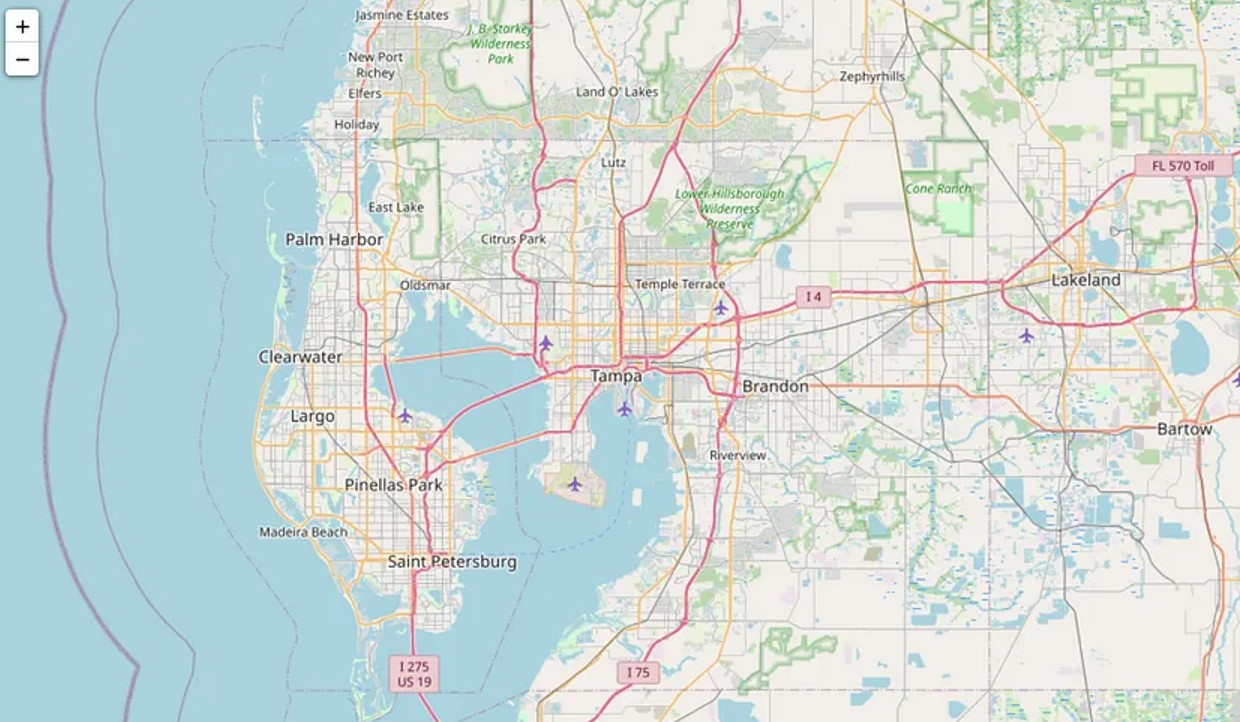
\includegraphics[width=0.65\textwidth]{3/figures/florida.jpg}
		\caption[Mapa de Tampa, Florida, creado en Folium y OpenStreetMap]{Mapa de Tampa, Florida, creado en Folium y OpenStreetMap\\
			Fuente: \citep*{gl_folium}. \citetitle{gl_folium}.}
		\label{1:fig}
	\end{center}
\end{figure}
\textbf{Entregable:} Visualización de la ruta segura seleccionada.

\begin{landscape}
	\section{Cronograma de actividades y presupuesto}
	Se elaboró un cronograma de actividades de toda la investigación, mostrada en la Figura \ref{1:fig1}, contemplando desde el inicio del mes de abril 2024 hasta la sustentación del trabajo estimado para inicios de diciembre 2024.
	
	\begin{figure}[!ht]
		\begin{center}
			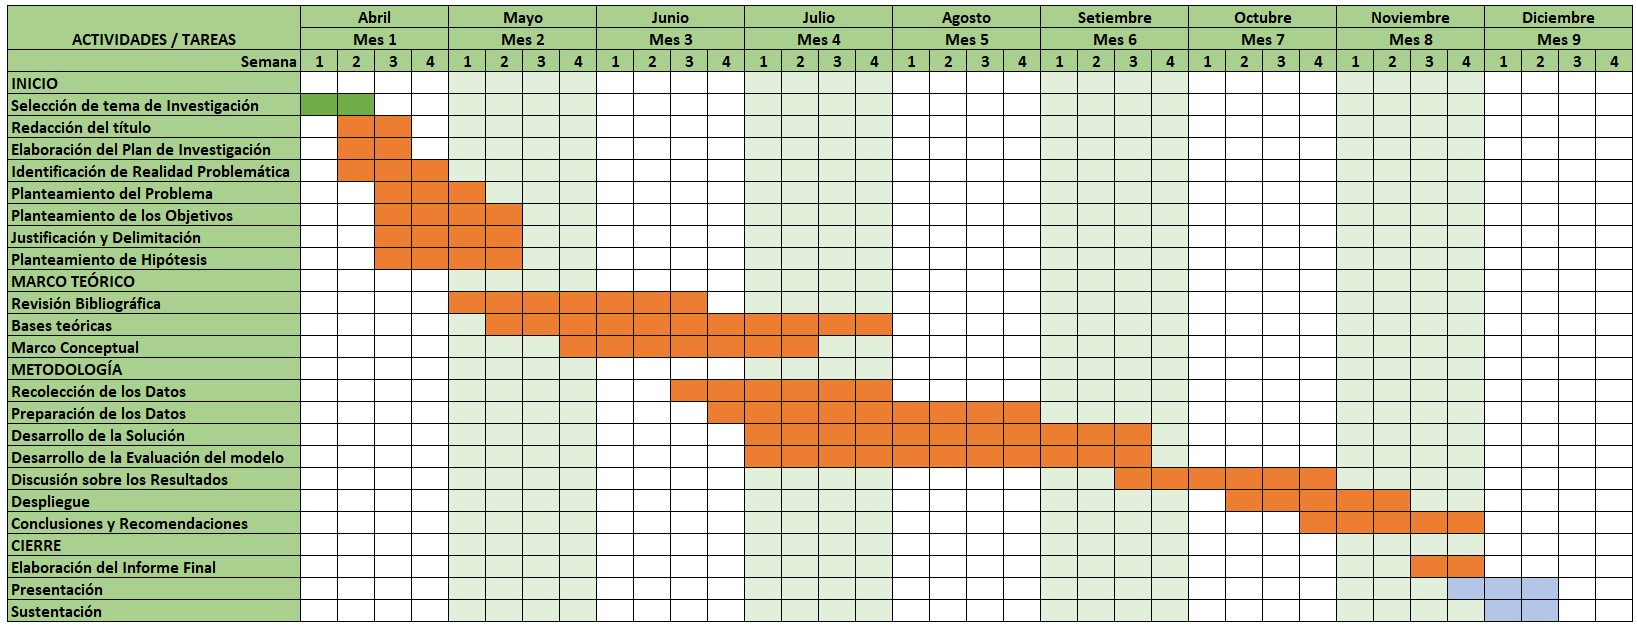
\includegraphics[width=1.55\textwidth]{3/figures/crono.jpg}
			\caption[Cronograma de actividades de la investigación]{Cronograma de actividades de la investigación.\\
				Fuente: Elaboración propia.}
			\label{1:fig1}
		\end{center}
	\end{figure}
	
\end{landscape}

A continuación, se muestra los costos personales del autor para la resolución del proyecto.

    \begin{table}[h!]
	\caption[Presupuesto de los costos personales del autor]{Presupuesto de los costos personales del autor.}
	\label{1:table}
	\centering
	\small
	\begin{tabular}{lcrr}
		\specialrule{.1em}{.05em}{.05em}
		\multicolumn{1}{c}{\centering{Item}} & \multicolumn{1}{c}{\centering{Tiempo usado (horas)}} & \multicolumn{1}{c}{\centering{Costo (soles)}} & \multicolumn{1}{c}{\centering{Subtotal}}
		\\
		\specialrule{.1em}{.05em}{.05em}
		\multicolumn{4}{l}{Recursos materiales}
		\\
		Laptop HP Pavilion Gaming Laptop 15 core i7 9750h 16GB  &  & S/.3,208.50 & S/.3,208.50
		\\
		\hline
		\multicolumn{4}{l}{Servicios generales}
		\\
		Internet + luz (9 meses) & \multicolumn{1}{r}{110} & S/.327.00 & S/.2,943.00
		\\
		\specialrule{.1em}{.05em}{.05em}
		Total &  &  & \multicolumn{1}{l}{S/.6,151.50}
		\\
		\specialrule{.1em}{.05em}{.05em}
	\end{tabular}
	\begin{flushleft}
		\small Fuente: Elaboración propia.
	\end{flushleft}
\end{table}
%\begin{table}[h]
%	\centering
%	\begin{tabular}{l|r}
%		Item & Quantity \\\hline
%		Widgets & 42 \\
%		Gadgets & 13
%	\end{tabular}
%	\caption{\label{tab:widgets}An example table.}
%\end{table}
%\chapter{DESARROLLO DEL EXPERIMENTO}
\section{X}

Hello, here is some text without a meaning.  This text should 
show what a printed text will look like at this place.  If you 
read this text, you will get no information.  Really?  Is there 
no information?  Is there a difference between this text and some 
nonsense like ``Huardest gefburn?  Kjift " not at all!...

\begin{table}
	\centering
	\begin{tabular}{l|r}
		Item & Quantity \\\hline
		Widgets & 42 \\
		Gadgets & 13
	\end{tabular}
	\caption{\label{tab:widgets1}An example table.}
\end{table}

\section{Y}

 Nisi porta lorem mollis aliquam ut porttitor leo. Aenean pharetra magna ac placerat vestibulum. Est placerat in egestas erat imperdiet sed euismod. Velit euismod in pellentesque massa placerat. Enim praesent elementum facilisis leo vel fringilla. Ante in nibh mauris cursus mattis molestie a iaculis. Erat pellentesque adipiscing commodo elit at imperdiet dui accumsan sit. Porttitor lacus luctus accumsan tortor posuere ac ut. Tortor at auctor urna nunc id. A iaculis at erat pellentesque adipiscing commodo elit. 


\section{Z}

Nisi porta lorem mollis aliquam ut porttitor leo. Aenean pharetra magna ac placerat vestibulum. Est placerat in egestas erat imperdiet sed euismod. Velit euismod in pellentesque massa placerat. Enim praesent elementum facilisis leo vel fringilla. Ante in nibh mauris cursus mattis molestie a iaculis. Erat pellentesque adipiscing commodo elit at imperdiet dui accumsan sit. Porttitor lacus luctus accumsan tortor posuere ac ut. Tortor at auctor urna nunc id. A iaculis at erat pellentesque adipiscing commodo elit. 

El paper es citado  y el otro paper .

%\chapter{ANÁLISIS Y DISCUSIÓN DE RESULTADOS}
\section{X}

Hello, here is some text without a meaning.  This text should 
show what a printed text will look like at this place.  If you 
read this text, you will get no information.  Really?  Is there 
no information?  Is there a difference between this text and some 
nonsense like ``Huardest gefburn?  Kjift " not at all!...

\begin{table}
	\centering
	\begin{tabular}{l|r}
		Item & Quantity \\\hline
		Widgets & 42 \\
		Gadgets & 13
	\end{tabular}
	\caption{\label{tab:widgetxcxs}An example table.}
\end{table}

\section{Y}

Nisi porta lorem mollis aliquam ut porttitor leo. Aenean pharetra magna ac placerat vestibulum. Est placerat in egestas erat imperdiet sed euismod. Velit euismod in pellentesque massa placerat. Enim praesent elementum facilisis leo vel fringilla. Ante in nibh mauris cursus mattis molestie a iaculis. Erat pellentesque adipiscing commodo elit at imperdiet dui accumsan sit. Porttitor lacus luctus accumsan tortor posuere ac ut. Tortor at auctor urna nunc id. A iaculis at erat pellentesque adipiscing commodo elit. 


\section{Z}

Nisi porta lorem mollis aliquam ut porttitor leo. Aenean pharetra magna ac placerat vestibulum. Est placerat in egestas erat imperdiet sed euismod. Velit euismod in pellentesque massa placerat. Enim praesent elementum facilisis leo vel fringilla. Ante in nibh mauris cursus mattis molestie a iaculis. Erat pellentesque adipiscing commodo elit at imperdiet dui accumsan sit. Porttitor lacus luctus accumsan tortor posuere ac ut. Tortor at auctor urna nunc id. A iaculis at erat pellentesque adipiscing commodo elit.

%\chapter{CONCLUSIONES Y RECOMENDACIONES}
\section{Conclusiones}

Hello, here is some text without a meaning.  This text should 
show what a printed text will look like at this place.  If you 
read this text, you will get no information.  Really?  Is there 
no information?  Is there a difference between this text and some 
nonsense like ``Huardest gefburn?  Kjift " not at all!...



\section{Recomendaciones}

Nisi porta lorem mollis aliquam ut porttitor leo. Aenean pharetra magna ac placerat vestibulum. Est placerat in egestas erat imperdiet sed euismod. Velit euismod in pellentesque massa placerat. Enim praesent elementum facilisis leo vel fringilla. Ante in nibh mauris cursus mattis molestie a iaculis. Erat pellentesque adipiscing commodo elit at imperdiet dui accumsan sit. Porttitor lacus luctus accumsan tortor posuere ac ut. Tortor at auctor urna nunc id. A iaculis at erat pellentesque adipiscing commodo elit. 



%%Anexos
\appendix
\renewcommand{\appendixname}{Anexos}
\renewcommand{\appendixtocname}{Anexos}
\renewcommand{\appendixpagename}{Anexos}
\clearpage
\addappheadtotoc
\appendixpage
\chapter{Anexo I: Matriz de Consistencia}


\begin{table}[h!]
	\centering
	\small
	\begin{tabular}{ |m{5cm}|m{5cm}|m{5cm}|  }
		\hline
		\rowcolor{bluejean}
		\Centering \color{white}{PROBLEMAS}& \Centering \color{white}{OBJETIVOS}& \Centering \color{white}{HIPÓTESIS}\\
		\hline
		\rowcolor{turq}
		\Centering Problema General& \Centering Objetivo General & \Centering Hipótesis General \\
		\hline
		{\ProblemaGeneral} & { \ObjetivoGeneral} & {\HipotesisGeneral} \\
		\hline
		\rowcolor{turq}
		\Centering Problemas Específicos& \Centering Objetivos Específicos & \Centering Hipótesis Específicas \\
		\hline
		{\Pbone} & {\Objone} & {\Hone} \\
		\hline
		{\Pbtwo} & {\Objtwo} & {\Htwo} \\
		\hline
		{\Pbthree} & {\Objthree} & {\Hthree} \\
		\hline
		{\Pbfour} & {\Objfour} & {\Hfour} \\
		\hline
		{\Pbfive} & {\Objfive} & {\Hfive} \\
		\hline
	\end{tabular}
	\caption{Matriz de consistencia. Fuente: Elaboración propia}
	\label{1:table}
\end{table}



\chapter{Anexo II: Resumen de Papers investigados}
%\section{Conclusiones}

\begin{table}[h]
	\newcommand{\multirot}[1]{\multirow{2}{*}[-8ex]{\rotcell{\rlap{#1}}}}
	%\scriptsize
	\footnotesize
	\centering
	\begin{tabular}{|m{0.5cm}|m{0.3cm}|m{4cm}|m{2cm}|m{0.6cm}|m{1.7cm}|m{3cm}|} 
		\hline
		\rowcolor[rgb]{0,0.251,0.502} \multicolumn{1}{|c|}{\textcolor{white}{Tipo}} & \multicolumn{1}{c|}{\textcolor{white}{N°}} & \multicolumn{1}{c|}{\textcolor{white}{Título}}                                                                             & \multicolumn{1}{c|}{\textcolor{white}{Autor}}        & \multicolumn{1}{c|}{\textcolor{white}{Año}} & \multicolumn{1}{c|}{\textcolor{white}{País}} & \multicolumn{1}{c|}{\textcolor{white}{Fuente}}                                                        \\ 
		\hline
		\multirot{Problema}                                        & 1                                             & Copper price estimation using bat algorithm~                                                                               & Dehghani  Bogdanovic                                 & 2018                                        & United Kingdom                               & Resources Policy                                                                                      \\ 
		\cline{2-7}
		& 2                                             & Alternative techniques for forecasting mineral commodity prices                                                            & Cortez, Saydam, Coulton,  Sammut                     & 2018                                        & Netherlands                                  & International Journal of Mining Science and Technology                                                \\ 
		\hline
		\multirow{3}{*}[-14ex]{\rotcell{\rlap{Propuesta}}}
		& 3                                             & Prediction of the crude oil price thanks to natural language
		processing applied to newspapers~                           & Trastour, Genin,  Morlot                             & 2016                                        & USA                                          & Standfort University ML repository                                                                    \\ 
		\cline{2-7}
		& 4                                             & Stock Price Prediction Using Deep Learning~                                                                                & Tipirisetty                                          & 2018                                        & USA                                          & Master's Theses San Jose State University                                                             \\ 
		\cline{2-7}
		& 5                                             & Deep Learning for Stock Prediction Using Numerical and Textual
		Information                                               & Akita, R., Yoshihara, A., Matsubara, T.,  Uehara, K. & 2016                                        & USA                                          & 2016 IEEE/ACIS 15th International Conference on Computer and
		Information Science (ICIS)             \\ 
		\hline
		\multirow{4}{*}[-28ex]{\rotcell{\rlap{Técnica}}}                                          & 6                                             & Stock Prices Prediction using the Title of Newspaper Articles
		with Korean Natural Language Processing~                   & Yun, Sim,  Seok                                      & 2019                                        & Japan                                        & 2019 International Conference on Artificial Intelligence in
		Information and Communication (ICAIIC)  \\ 
		\cline{2-7}
		& 7                                             & A Method of Optimizing LDA Result Purity Based on Semantic
		Similarity                                                    & Jingrui, Z., Qinglin, W., Yu, L.,  Yuan, L.          & 2017                                        & China                                        & 2017 32nd Youth Academic Annual Conference of Chinese
		Association of Automation (YAC)~              \\ 
		\cline{2-7}
		& 8                                             & Qualitative Stock Market Predicting with Common Knowledge Based
		Nature Language Processing: A Unified View and Procedure & Rao, D., Deng, F., Jiang, Z.,  Zhao, G.~             & 2015                                        & USA                                          & 2015 7th International Conference on Intelligent Human-Machine
		Systems and Cybernetics              \\ 
		\cline{2-7}
		& 9                                             & Fuzzy Bag-of-Words Model for Document Representation                                                                       & Zhao, R.,  Mao, K.                                   & 2018                                        & USA                                          & IEEE Transactions on Fuzzy Systems (~Volume:
		26~,~Issue: 2~, April 2018~)                           \\
		\hline
	\end{tabular}
	\caption{Cuadro Resumen de Papers investigados. Fuente: Elaboración propia}
\label{A:table}
\end{table}





% %%Bibliografia
%\bibliographystyle{apalike} % Title is link if provided
\renewcommand{\bibname}{BIBLIOGRAFÍA} % changes the header; default: Bibliography

\printbibliography[heading=bibintoc,title={BIBLIOGRAFÍA}]
%\bibliography{biblio/references} % adjust this to fit your BibTex file
\end{document}